\titleformat{\chapter}[display]{\bfseries\centering}{\huge Chapter \thechapter}{1em}{\Huge #1}
\newgeometry{top=3cm, bottom=2.2cm, left=3cm, right=2cm, headsep=1.2cm, footskip=1cm, headheight=0.3cm, textheight=24.5cm, textwidth=16cm}
\onehalfspacing
\pagestyle{fancy}
\fancyhf{}
\renewcommand{\headrulewidth}{0pt}
\lhead{Chapter 3}
\rhead{Proposed System}
\cfoot{\thepage}
\chapter{Proposed System}

\section{Detailed Explanation of the Proposed System}
\noindent Sentinel is organised as five layers (Figure~\ref{fig:arch}). The \textbf{input layer} is the four-page web application and the Chrome extension, which accept a message, a URL, ordered conversation turns, profile facts or an account, or read visible page text when auto-scan is on. The \textbf{preprocessing layer} validates each request, parses URLs without visiting them and builds the target message with its preceding turns. The \textbf{threat-detection layer} runs independent analysers: fraud rules, harm rules, the learned scam-text model, the community matcher, profile indicators and bot detection. The \textbf{security-analysis layer} assigns each analyser's level and keeps the results separate, and the \textbf{output layer} shows them in the web app, the extension popup or as page markers and, on request, saves the case. Supporting stores and services (the case store, checksummed model artifacts, the community hub and official platform APIs) sit beside the server.

\noindent\textbf{Workflow.} (1) The user pastes content into the web app, selects text or a link and opens the extension, turns on auto-scan for a site, or enters an account on the Bot accounts page. (2) The local API validates the request and runs the available analysers; links are never opened and profiles are never scraped. (3) The user reads each assessment with its observations, missing checks and uncertainty, or sees markers on risky page items. (4) The user verifies through an official channel and may save the case, add feedback, export it as JSON or delete it. If they opted in, a high-confidence scam is shared with the community hub as an anonymous fingerprint.\\

\noindent\textbf{Working principle.} Sentinel separates \emph{observation} from \emph{conclusion}. Each analyser produces short evidence statements (for example, ``The message asks for a password or verification code''); its level is derived from the evidence by fixed rules, and every result lists the checks that could not be performed, so a missing check is never read as a safe result. A learned model is attached only from a checksum-verified artifact and only after it has passed a release gate fixed before training; its output appears in its own block and never changes the rule-based fraud or harm level. A model that fails its gate, or fails at run time, is reported as \emph{unavailable} or \emph{research only}, and the rules still answer. In the research pipeline every model is trained, tuned, calibrated and evaluated on separate partitions, the last made of unseen domains, templates, datasets or bot families (Section~\ref{sec:algos}).

\begin{figure}[H]
\centering
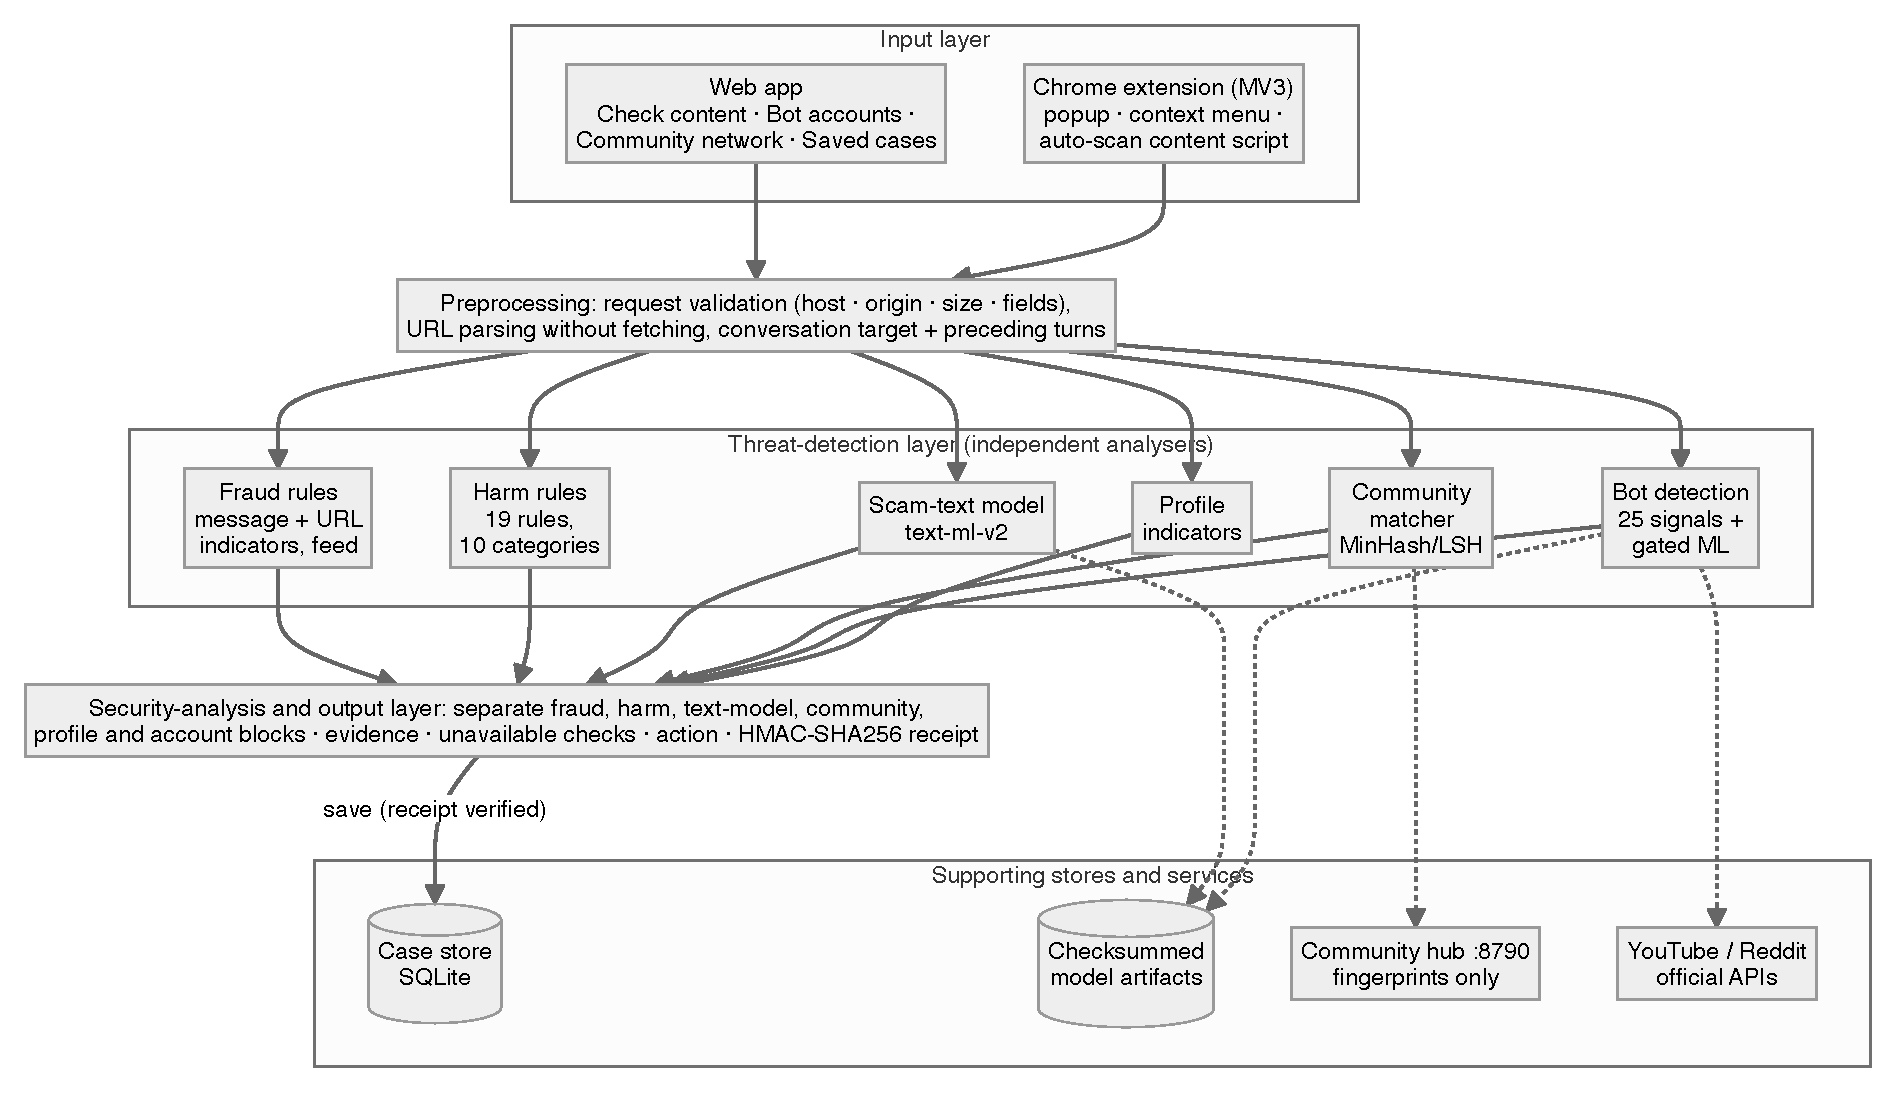
\includegraphics[width=\linewidth]{dia2/arch_v2.pdf}
\caption{Layered architecture of Sentinel (dashed arrows: optional supporting stores and services)}
\label{fig:arch}
\end{figure}

\subsection{Module-wise Explanation}
\begin{enumerate}[label=\textbf{M\arabic*}, leftmargin=1.2cm]
\item \textbf{Web client (\texttt{web/}):} four pages sharing one navigation bar. \emph{Check content} has fields for a message, a URL, an ordered conversation editor (linear or reply threads, with a selectable target turn) and optional profile facts, and shows one card per assessment, moving the harm card to the top when it is high. \emph{Bot accounts} accepts a profile link, an upload or manual entry and draws a score gauge and signal list. \emph{Community network} shows the hub's live campaigns and statistics, and \emph{Saved cases} lists stored cases. All text is inserted with \texttt{textContent}, never as HTML, as the Content-Security-Policy requires.
\item \textbf{Chrome extension (\texttt{extension/}, Manifest V3):} a popup and ``Check selected text'' and ``Check link'' context-menu items for on-demand checks, and \emph{auto-scan}. When the user turns auto-scan on for a site, the extension requests that site's host permission with \texttt{chrome.permissions\allowbreak.request} and registers the content script \texttt{scanner.js} for it only. The script finds visible text with an \texttt{IntersectionObserver}, catches new content with a \texttt{MutationObserver} (800 ms debounce), groups and de-duplicates text units and sends batches of at most 25 to the background service worker, which relays them to \texttt{POST /api/scan} with an 8-second timeout. Results are drawn as markers in a shadow-DOM overlay that page styles cannot reach, and the toolbar badge counts high and review items. If the server is unreachable the scanner pauses for 15 seconds and retries; it never shows anything as ``safe''.
\item \textbf{Local API and request validation (\texttt{server.py}):} a threaded standard-library HTTP server on the loopback interface that rejects a non-local \texttt{Host}, accepts browser origins only from itself and Chrome extensions, requires \texttt{application/json}, limits bodies to 200,000 bytes (3 MB for bot uploads), and sends the headers \texttt{Content-Security-Policy:} \texttt{default-src 'self'}, \texttt{X-Content-Type-\allowbreak Options: nosniff} and \texttt{Cache-Control: no-store} (endpoints in Appendix-I). An optional component that fails yields an ``unavailable'' block; the request still succeeds.
\item \textbf{Fraud (message and link) checker (\texttt{analysis.py}):} regular expressions for payment or fees, passwords/OTPs/verification codes and urgency; URL indicators (``@'' in the authority, punycode, IP-address host, four or more dots in the host, length above 180); and an exact match in an optional verified phishing CSV as the strongest evidence.
\item \textbf{Harmful-language rule engine (\texttt{harm\_rules.py}):} 19 rules in 10 categories. High: threats of violence, mass violence, self-harm encouragement, self-harm risk, sextortion, blackmail, doxxing and stalking, and dehumanising hate. Review: harassment and directed insults, including Hinglish. Low: profanity, which is not flagged. Text is first normalised (NFKC, look-alike letters, dotted letters joined, leetspeak inside words, stretched letters collapsed); idioms are skipped, a negation shortly before a match lowers it, and quoted or reported speech lowers \emph{high} to \emph{review}, except self-harm risk, which is never downgraded. Advice follows a fixed priority, with Tele-MANAS (14416) and emergency (112) numbers for self-harm \cite{telemanas}. The earlier three-phrase rule is kept only as a frozen baseline for research evaluation.
\item \textbf{Learned scam-text model (\texttt{text\_ml/}, text-ml-v2):} a DistilBERT classifier \cite{distilbert} fine-tuned on SMS into ham, spam and smishing, exported to ONNX \cite{onnx}, averaged with a TF-IDF word and character n-gram logistic regression \cite{sklearn}, and calibrated by temperature scaling. A message is flagged when its scam probability reaches 0.611, and each flag is explained by the words whose removal most lowers the scam log-odds. The artifact's files are verified against SHA-256 checksums before loading.
\item \textbf{Batch scan (\texttt{scan.py}):} the auto-scan endpoint. It accepts at most 40 items of up to 4,000 characters, runs the fraud and harm rules on each, checks whether a link's visible text names a different site than its destination, scores all items with the text model in one batch (explaining at most five), adds community matches and assigns a severity of \emph{high}, \emph{review} or \emph{none} (Algorithm~\ref{alg:scan}).
\item \textbf{Community scam network (\texttt{network/}):} each client turns a high-confidence scam into a fingerprint (a 64-value MinHash of word 3-grams of the masked template, 32 LSH band keys, salted domain hashes and fixed topic tags) and, if the user opted in, reports it from a background thread. The hub (\texttt{hub.py}, \texttt{hub\_server.py}, port 8790) clusters reports and publishes a campaign after $k=5$ distinct reporters, with rate limits, half weight for new clients, reputation, a verified-sender allowlist, disputes and 24-hour decay. Clients download the campaign feed and match incoming messages locally, so the hub never sees message text. \texttt{simulate.py} and \texttt{experiments.py} run the agent-based simulation.
\item \textbf{Bot-account detection (\texttt{bot\_detection/}):} profile links are parsed against an exact host allowlist and never fetched, so they cannot be used for server-side request forgery. Data comes from the YouTube Data API or the Reddit API (keys read only from environment variables; HTTPS to three fixed hosts, no redirects, 10-second timeout, 2 MB cap), or from a JSON/CSV upload or manual entry. Profile, activity, content and engagement features feed a 25-signal weighted heuristic and two trained models: the profile model \emph{bot-ml-v1} (withheld, failed its gate) and the activity model \emph{bot-ml-activity-v1} (released for X accounts with at least 20 timed posts). Analyses are rate-limited to 12 per minute and logs never contain usernames.
\item \textbf{Profile indicator checker:} at least 50 posts in 24 hours; following at least 500 accounts and more than twenty times its followers; a website host that differs from a supplied official domain. In the content check, bot likelihood is reported as ``not estimated''; the bot-detection module (M9) is the place for that estimate.
\item \textbf{Result assembly and receipts (\texttt{assessment\_receipts.py}):} returns the separate assessment blocks and a receipt, an HMAC-SHA256 \cite{hmac} over the exact input and result with a per-process 32-byte key, valid for 15 minutes. A reviewed result is saved only with a valid receipt.
\item \textbf{Case store (\texttt{storage.py}):} saved cases in a local SQLite table with feedback (correct, incorrect, unsure), JSON export and deletion. Feedback is never used for training automatically.
\item \textbf{ML research pipeline:} command-line tools that acquire checksum-verified datasets, audit duplicates and label conflicts, freeze grouped splits, check data-support gates, fit models in memory-capped processes, select on validation or calibration data, calibrate and evaluate once. Study families: URL classification (versions 1--3), the scam-text model (v1 and v2), bot detection (profile and activity models), the community-network simulation, paired message--link detection and contextual directed abuse.
\end{enumerate}

\section{System Analysis}
\subsection{Functional Requirements}
\begin{enumerate}[label=FR\arabic*:, leftmargin=1.4cm]
\item Accept a message, a URL (up to 2,048 characters), ordered conversation turns with a selected target, and profile facts, individually or together.
\item Reject an empty or non-JSON request, a body over 200,000 bytes and invalid profile values with a clear error.
\item Assess fraud, harmful content and profile indicators separately, each with a level or status, evidence, unavailable checks, uncertainty and a suggested action.
\item Never fetch the submitted URL or scrape a profile.
\item Optionally load a verified phishing CSV; report exact matches as evidence and other links as unlisted.
\item Save a reviewed result only with a valid, unexpired receipt for that exact input and result.
\item List saved cases and allow feedback, JSON export and deletion.
\item Let the Chrome extension check selected text or a link after a user action, and scan visible page text only on sites the user has turned auto-scan on for, through the same API.
\item Detect harmful language in English and Hinglish, report its categories and give advice by fixed priority, with support numbers for self-harm.
\item Report the learned scam-text model in its own block with a calibrated probability, the threshold and the words that drove a flag.
\item Assign each scanned page item a severity of high, review or none and draw markers without changing the page.
\item Share only anonymous fingerprints with the community hub, only when the user opts in; publish a campaign only after five distinct reporters; match the campaign feed locally.
\item Analyse an account from official APIs, an upload or manual entry; reject profile URLs with credentials, ports or unknown hosts; withhold the score when data coverage is too low; show a trained model's estimate only if it passed its gate.
\item Freeze grouped splits, select models on validation or calibration data only and evaluate each frozen model once (research tools).
\end{enumerate}

\subsection{Non-Functional Requirements}
\begin{itemize}
\item \textbf{Privacy:} analysis runs on the user's machine; nothing is stored unless saved; the community hub stores fingerprints, counts and times but never message text; bot-detection logs omit usernames; research data stay in Git-ignored local storage.
\item \textbf{Security:} loopback-only binding, host and origin checks, size limits, CSP headers, text-only rendering, signed save receipts, SSRF-safe account parsing, rate limits and API keys only from environment variables.
\item \textbf{Explainability:} every result states its evidence, missing checks and uncertainty in plain language.
\item \textbf{Performance:} a rule-based analysis completes in milliseconds and the scam-text model takes about 1.9 ms per message batched on a laptop CPU; URL training fits an 8 GiB memory ceiling.
\item \textbf{Reproducibility and maintainability:} pinned dependencies, fixed seeds, SHA-256 manifests, modular packages and automated Python and JavaScript tests.
\item \textbf{Portability:} the rules-only application needs only Python 3.10+ and a browser, on Windows, macOS or Linux; the learned models add ONNX Runtime, \texttt{tokenizers}, scikit-learn and NumPy.
\item \textbf{Fail-safety:} a missing, tampered or failing model, an unreachable hub or an upstream API error produces an ``unavailable'' block or a clear error, never a silent ``safe'' result.
\end{itemize}

\subsection{Specific Requirements}
\noindent A learned model is shown live only after it passes a release gate fixed before training (text-ml-v2 and bot-ml-activity-v1 passed; the URL models and bot-ml-v1 did not and stay in research); the self-harm category is never downgraded; a link absent from the feed is reported as unlisted, never safe; spam/ham labels are not relabelled as phishing and historical labels are not presented as verification of current websites; and user feedback is never added to training data automatically.

\subsection{Software and Hardware Requirements}
\begin{table}[H]
\centering
\small
\renewcommand{\arraystretch}{1.25}
\caption{Software and hardware requirements}
\label{tab:swhw}
\begin{tabular}{|>{\raggedright\arraybackslash}p{3.7cm}|>{\raggedright\arraybackslash}p{11.1cm}|}
\hline
\textbf{Component} & \textbf{Requirement} \\ \hline
Operating system & Windows 10/11, macOS or Linux \\ \hline
Application runtime & Python 3.10 or newer, standard library only (rules-only mode); SQLite bundled with Python \\ \hline
Model runtime & \texttt{.venv-text-ml} (CPython 3.13): ONNX Runtime 1.31, \texttt{tokenizers} 0.23, scikit-learn 1.9.1, NumPy; PyTorch and Transformers for training only \\ \hline
Research runtime & CPython 3.11 with pinned locks: NumPy, SciPy, scikit-learn 1.9.1, joblib, tldextract, psutil, PyArrow; optional encoder lock with PyTorch 2.8 and Transformers 4.57 \\ \hline
Browser and testing & Google Chrome (Developer mode for the unpacked extension); Python \texttt{unittest}; Node.js 22+ for web-client tests \\ \hline
Hardware & AMD Ryzen 7 7435HS, 16 GiB RAM, optional NVIDIA RTX 3050 Laptop GPU (4 GiB VRAM); Apple M4 (MPS) used to fine-tune the scam-text model \\ \hline
Network & Not needed for content checks; loopback only for the community hub; internet only for the optional YouTube/Reddit APIs and to download research datasets \\ \hline
\end{tabular}
\end{table}

\subsection{Use Case Modelling}
\noindent Figure~\ref{fig:usecase} shows the actors and use cases: the \emph{User} checks content, views evidence and manages saved cases; the \emph{Research team member} runs the data and model pipeline; the \emph{Phishing feed} is a secondary system actor. The diagram covers the core check; the use cases added in this phase (auto-scan and account analysis, with the community hub and platform APIs as secondary actors) are given as templates in Tables~\ref{tab:uc4} and \ref{tab:uc5}, after the three original ones (Tables~\ref{tab:uc1}--\ref{tab:uc3}).
\begin{figure}[!htbp]
\centering
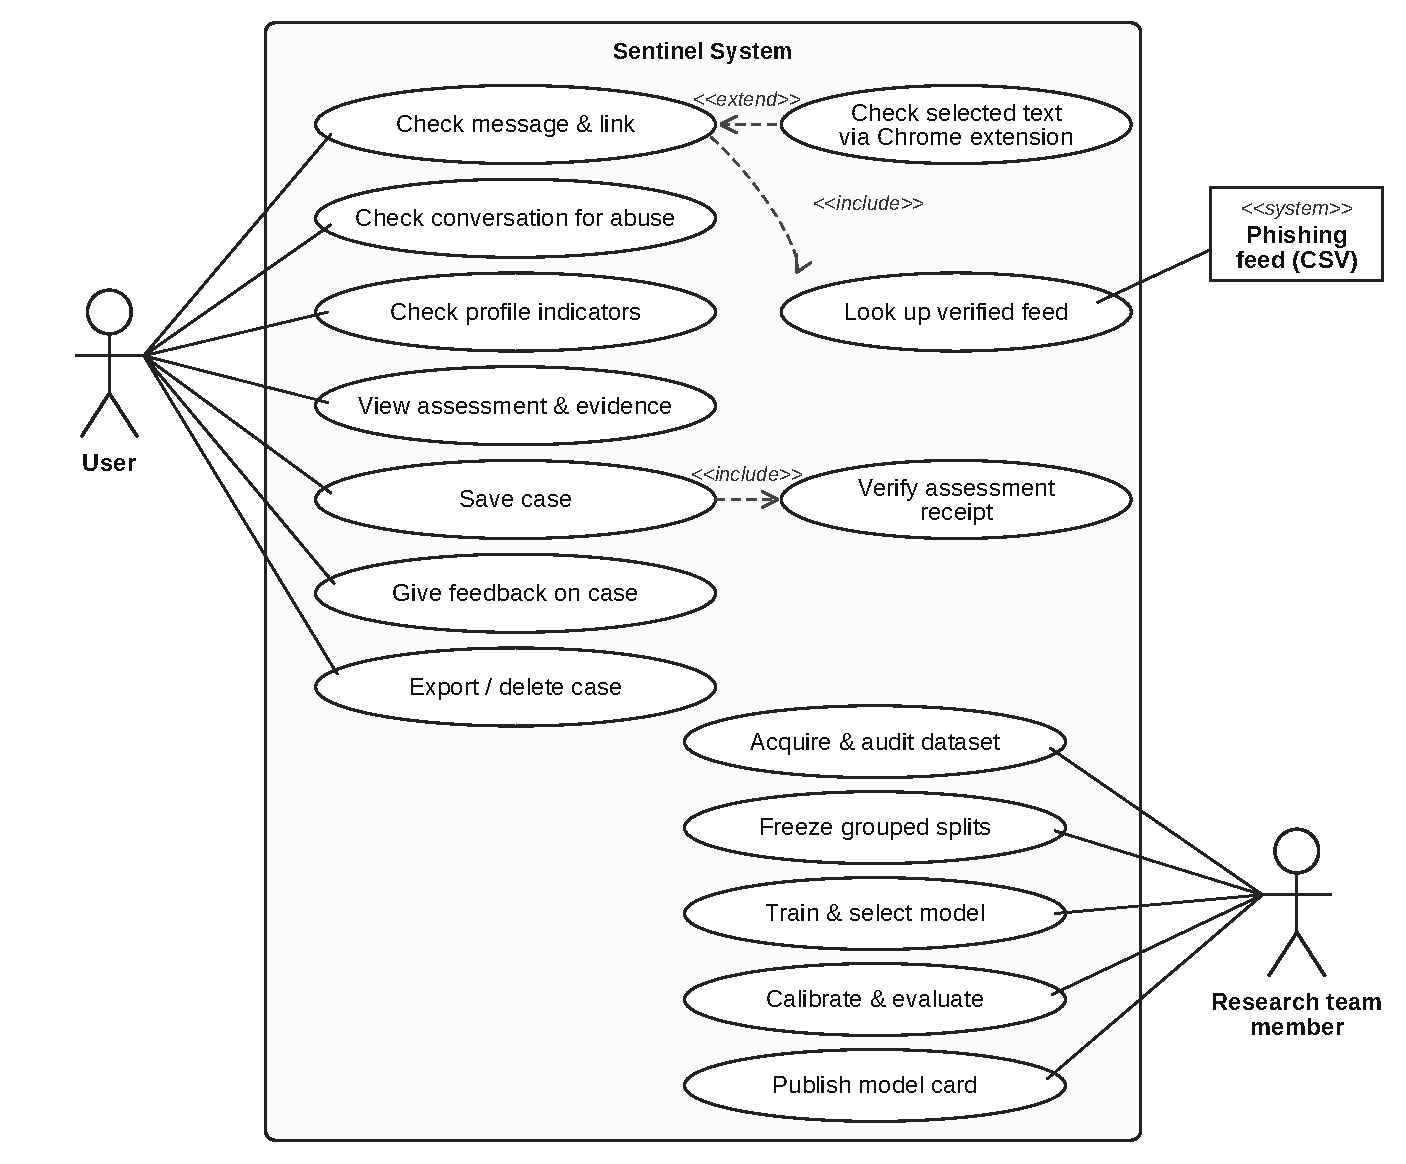
\includegraphics[width=\linewidth]{dia/usecase.pdf}
\caption{Use case diagram}
\label{fig:usecase}
\end{figure}

\begin{table}[H]
\centering
\footnotesize
\renewcommand{\arraystretch}{1.2}
\caption{Use case template: UC-01 Check message and link}
\label{tab:uc1}
\begin{tabular}{|>{\raggedright\arraybackslash}p{2.9cm}|>{\raggedright\arraybackslash}p{12.0cm}|}
\hline
\textbf{Actors} & Primary: User. Secondary: Phishing feed (optional) \\ \hline
\textbf{Description} & The user checks a suspicious message and its link before acting on it. \\ \hline
\textbf{Pre-conditions} & The local Sentinel service is running; the web app or extension is open. \\ \hline
\textbf{Main flow} & 1. User pastes or selects the message and/or link. 2. User clicks \emph{Analyze}. 3. API validates host, origin, size and fields. 4. Rules check payment, OTP and urgency wording and URL structure; feed lookup if loaded. 5. Harmful-content and profile checks run on any supplied data. 6. API returns assessments and a signed receipt. 7. UI shows level, evidence, missing checks and action. \\ \hline
\textbf{Alternate flows} & 3a. Invalid input: an error is shown and nothing is analysed. 4a. Feed not loaded: the result states that the reputation check is unavailable. \\ \hline
\textbf{Post-conditions} & Assessment is displayed; nothing is stored. \\ \hline
\end{tabular}
\end{table}

\begin{table}[H]
\centering
\footnotesize
\renewcommand{\arraystretch}{1.2}
\caption{Use case template: UC-02 Save case}
\label{tab:uc2}
\begin{tabular}{|>{\raggedright\arraybackslash}p{2.9cm}|>{\raggedright\arraybackslash}p{12.0cm}|}
\hline
\textbf{Actors} & Primary: User \\ \hline
\textbf{Description} & The user keeps a reviewed assessment for later reference or reporting. \\ \hline
\textbf{Pre-conditions} & UC-01 completed; input unchanged since the check; receipt less than 15 minutes old; service not restarted. \\ \hline
\textbf{Main flow} & 1. User clicks \emph{Save this case}. 2. Client sends input, result and receipt. 3. API verifies the HMAC and both hashes. 4. The case is inserted into SQLite with an ID and UTC timestamp. 5. UI confirms ``Saved locally'' and lists the case under Saved cases. \\ \hline
\textbf{Alternate flows} & 3a. Receipt invalid, expired or input edited: the user is asked to recheck. \\ \hline
\textbf{Post-conditions} & The case can be opened, marked, exported as JSON or deleted. \\ \hline
\end{tabular}
\end{table}

\begin{table}[H]
\centering
\footnotesize
\renewcommand{\arraystretch}{1.2}
\caption{Use case template: UC-03 Train and evaluate URL model}
\label{tab:uc3}
\begin{tabular}{|>{\raggedright\arraybackslash}p{2.9cm}|>{\raggedright\arraybackslash}p{12.0cm}|}
\hline
\textbf{Actors} & Primary: Research team member \\ \hline
\textbf{Description} & Produce a reproducible, held-out measurement of a URL classifier. \\ \hline
\textbf{Pre-conditions} & Research environment installed from pinned locks; dataset source and checksum pinned in the config. \\ \hline
\textbf{Main flow} & 1. Acquire and verify the source file. 2. Canonicalise and audit URLs. 3. Freeze grouped train/validation/calibration/test splits. 4. Check support gates. 5. Fit the grid in isolated processes. 6. Select by validation recall at $\le$5\% FPR. 7. Calibrate. 8. Export a checksummed artifact. 9. Evaluate once on the test split and publish a model card. \\ \hline
\textbf{Alternate flows} & 4a. A gate fails: stop and record a negative status, with no model or score. 9a. A frozen protocol was already scored: further fitting is refused. \\ \hline
\textbf{Post-conditions} & Metrics, intervals and limitations are published; the model is served only if it passed its gate. \\ \hline
\end{tabular}
\end{table}

\begin{table}[H]
\centering
\footnotesize
\renewcommand{\arraystretch}{1.2}
\caption{Use case template: UC-04 Auto-scan a page}
\label{tab:uc4}
\begin{tabular}{|>{\raggedright\arraybackslash}p{2.9cm}|>{\raggedright\arraybackslash}p{12.0cm}|}
\hline
\textbf{Actors} & Primary: User. Secondary: Community hub (optional) \\ \hline
\textbf{Description} & While browsing a chat or social site, the user is warned about risky visible messages. \\ \hline
\textbf{Pre-conditions} & Sentinel is running; the extension is installed; the user turned auto-scan on for this site and granted its host permission. \\ \hline
\textbf{Main flow} & 1. The content script collects visible text units and new content. 2. Units are de-duplicated and sent in batches of at most 25 through the background worker. 3. \texttt{/api/scan} runs rules, harm rules, the link-text check, the text model and community matching. 4. Each item gets a severity, evidence and an action. 5. High and review items are marked in an overlay and counted on the toolbar badge. \\ \hline
\textbf{Alternate flows} & 3a. Server unreachable: scanning pauses for 15 s and retries; nothing is shown as safe. 1a. Auto-scan turned off: the script is unregistered and markers are removed. \\ \hline
\textbf{Post-conditions} & Markers are shown; the page is unchanged; nothing is stored. \\ \hline
\end{tabular}
\end{table}

\begin{table}[H]
\centering
\footnotesize
\renewcommand{\arraystretch}{1.2}
\caption{Use case template: UC-05 Analyse an account for bot behaviour}
\label{tab:uc5}
\begin{tabular}{|>{\raggedright\arraybackslash}p{2.9cm}|>{\raggedright\arraybackslash}p{12.0cm}|}
\hline
\textbf{Actors} & Primary: User. Secondary: YouTube Data API or Reddit API (optional) \\ \hline
\textbf{Description} & The user checks whether an account behaves like an automated or fake account. \\ \hline
\textbf{Pre-conditions} & Sentinel is running; for the API source, the platform key is set in an environment variable. \\ \hline
\textbf{Main flow} & 1. User enters a profile link or handle and chooses API, upload or manual entry. 2. The link is parsed against the platform allowlist. 3. Data is fetched from the official API or read from the upload. 4. Features are extracted; the heuristic scores 25 signals. 5. A released model adds a separate probability line. 6. The report shows score, confidence, top signals and limitations. \\ \hline
\textbf{Alternate flows} & 2a. Hostile or unknown link: rejected before any network access. 3a. Key missing or API error: a clear error (400/502); 429 when rate-limited. 4a. Coverage below 25\% or fewer than 4 signals: the score is withheld. \\ \hline
\textbf{Post-conditions} & The report is displayed; nothing is stored. \\ \hline
\end{tabular}
\end{table}

\section{Proposed System: Analysis, Modelling and Design}
\noindent The applicable UML diagrams are the activity, sequence, class and deployment diagrams. The activity, first sequence, class, ER and data-flow diagrams describe the core content check, which is unchanged in structure; a second sequence diagram covers auto-scan, and the deployment diagram shows every component added in this phase. Statechart, collaboration and component diagrams are not included: a saved case only gains optional feedback before it is deleted, the sequence diagrams already show the object interactions, and the deployed components appear in the deployment diagram.

\subsection{Activity Diagram}
\noindent Figure~\ref{fig:activity} shows a check from input to optional saving. The server first checks host and origin, content type and size; the fields are then validated, the checkers run independently and are joined before the result is assembled.
\begin{figure}[H]
\centering
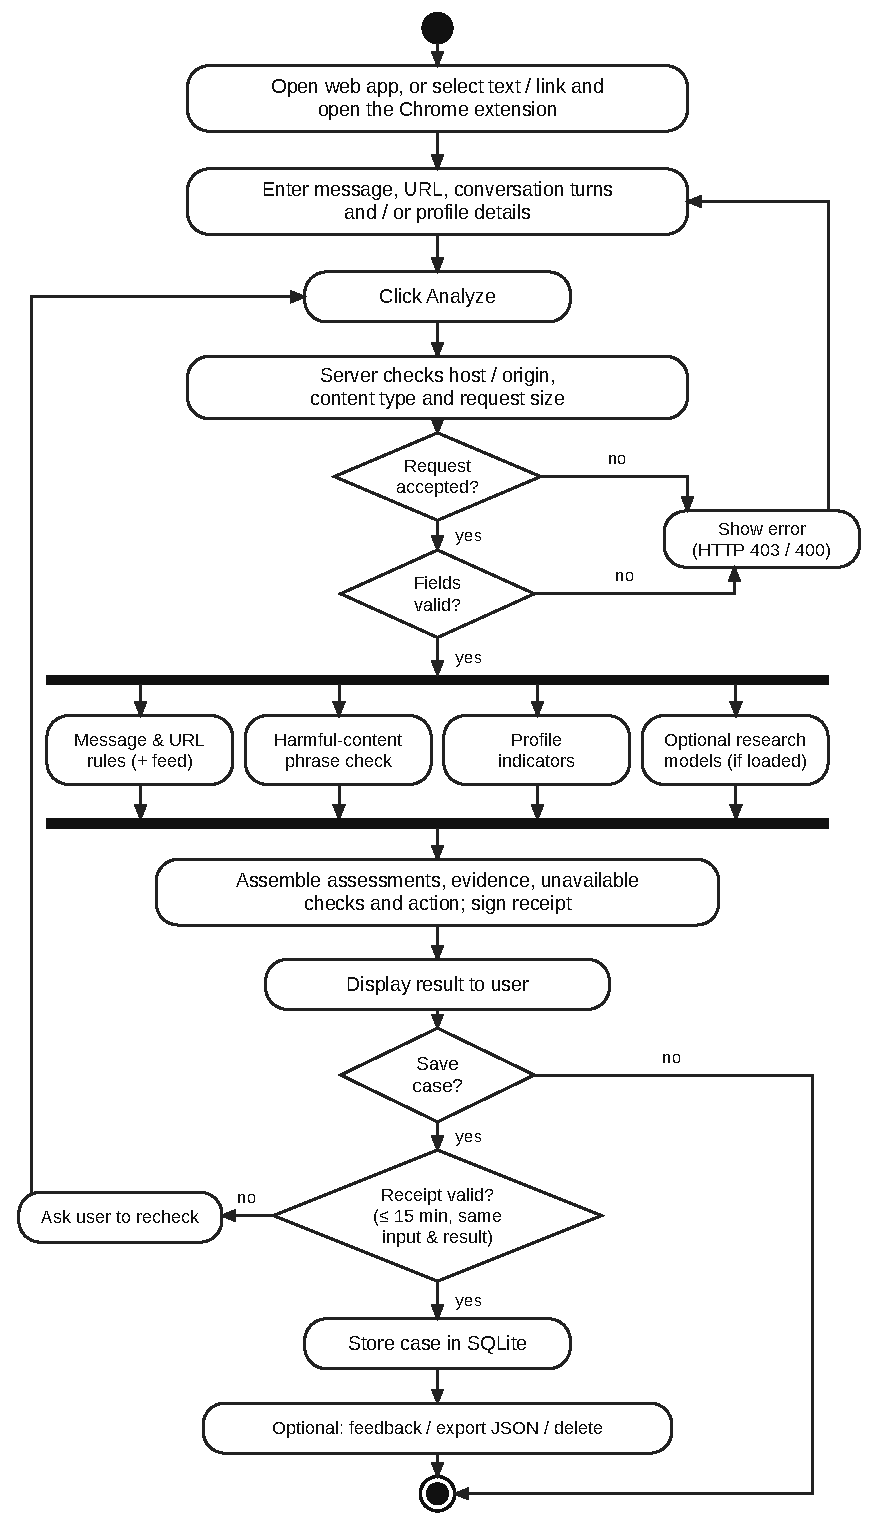
\includegraphics[height=0.78\textheight]{dia/activity.pdf}
\caption{Activity diagram of a Sentinel check}
\label{fig:activity}
\end{figure}

\subsection{Sequence Diagram}
\noindent Figure~\ref{fig:sequence} shows two interactions. In the first, the handler checks host and origin, reads and size-checks the JSON body, calls \texttt{analyze()}, obtains a receipt from \texttt{SnapshotSigner} and returns both. In the second, the receipt is verified before \texttt{CaseStore} inserts the record.
\begin{sidewaysfigure}
\centering
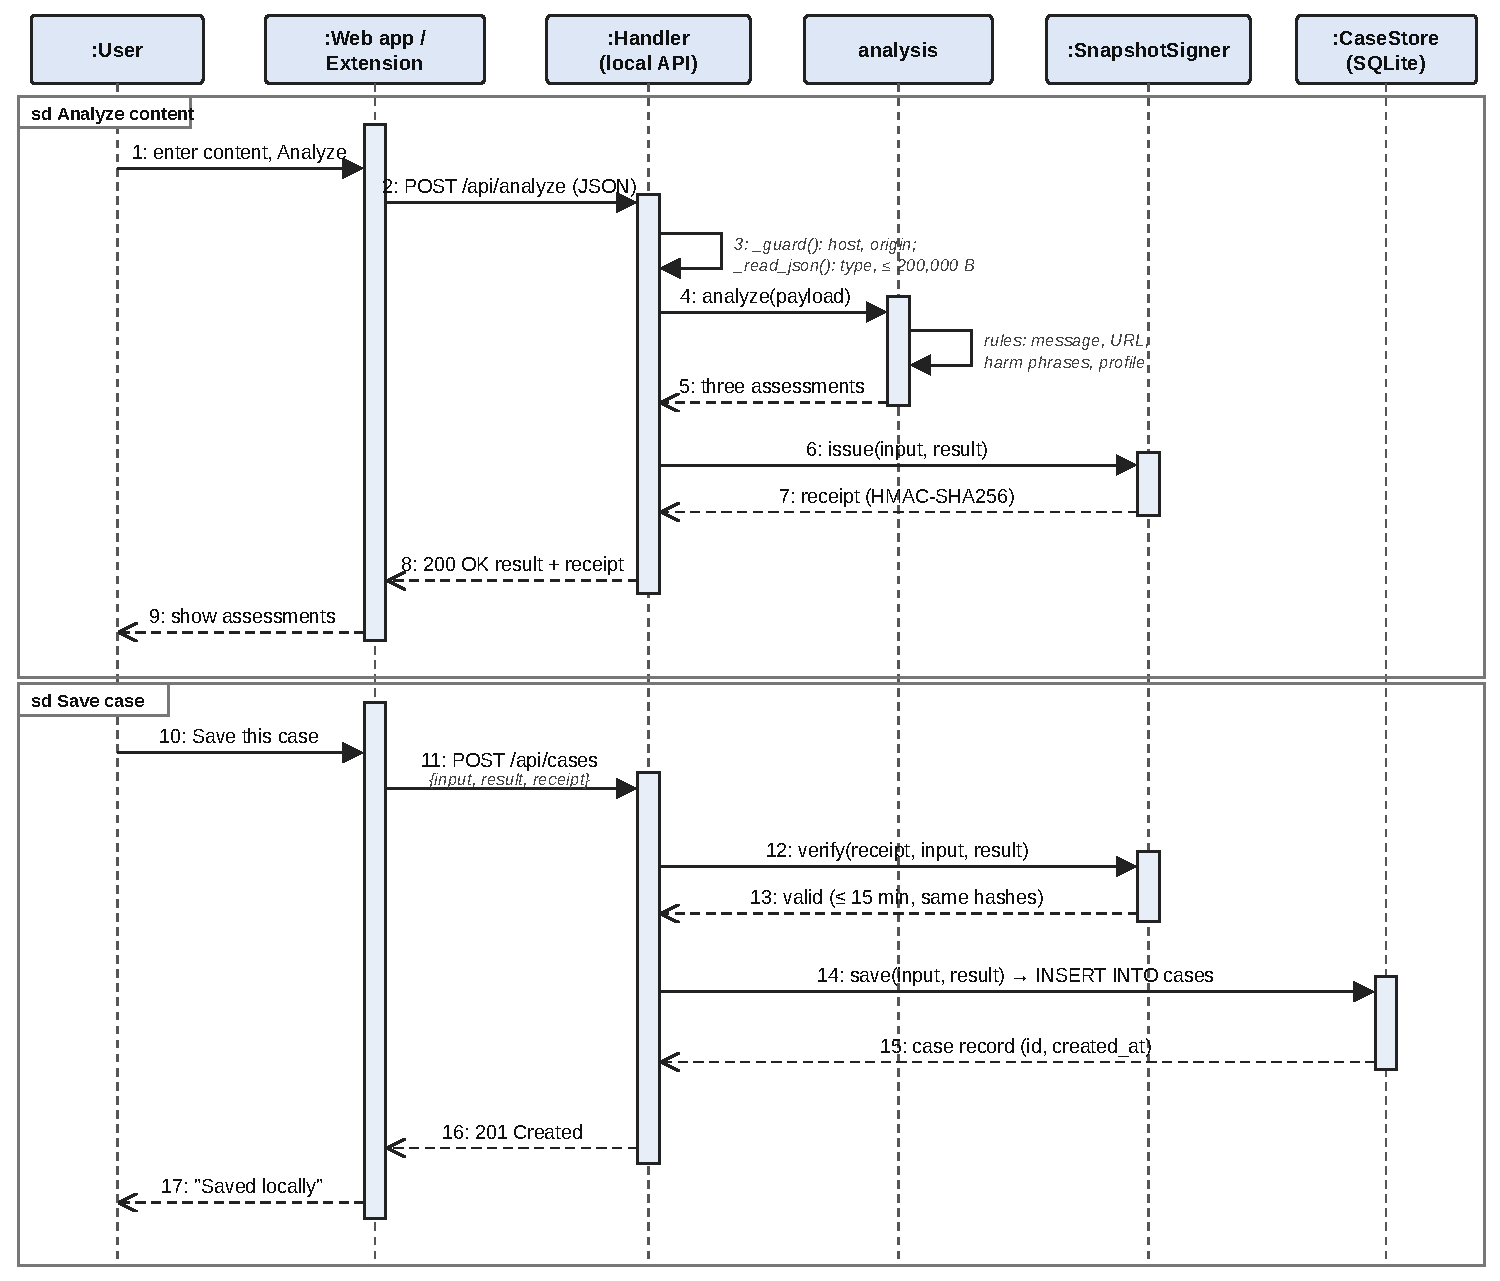
\includegraphics[width=\textheight]{dia/sequence.pdf}
\caption{Sequence diagram: analysing content and saving a case}
\label{fig:sequence}
\end{sidewaysfigure}

\noindent Figure~\ref{fig:autoscan} shows auto-scan. The user's switch in the popup grants the site permission and registers the content script; from then on, visible and newly added text is batched, relayed by the background worker and scored by \texttt{/api/scan}, and the results come back as markers and a badge count.
\begin{figure}[H]
\centering
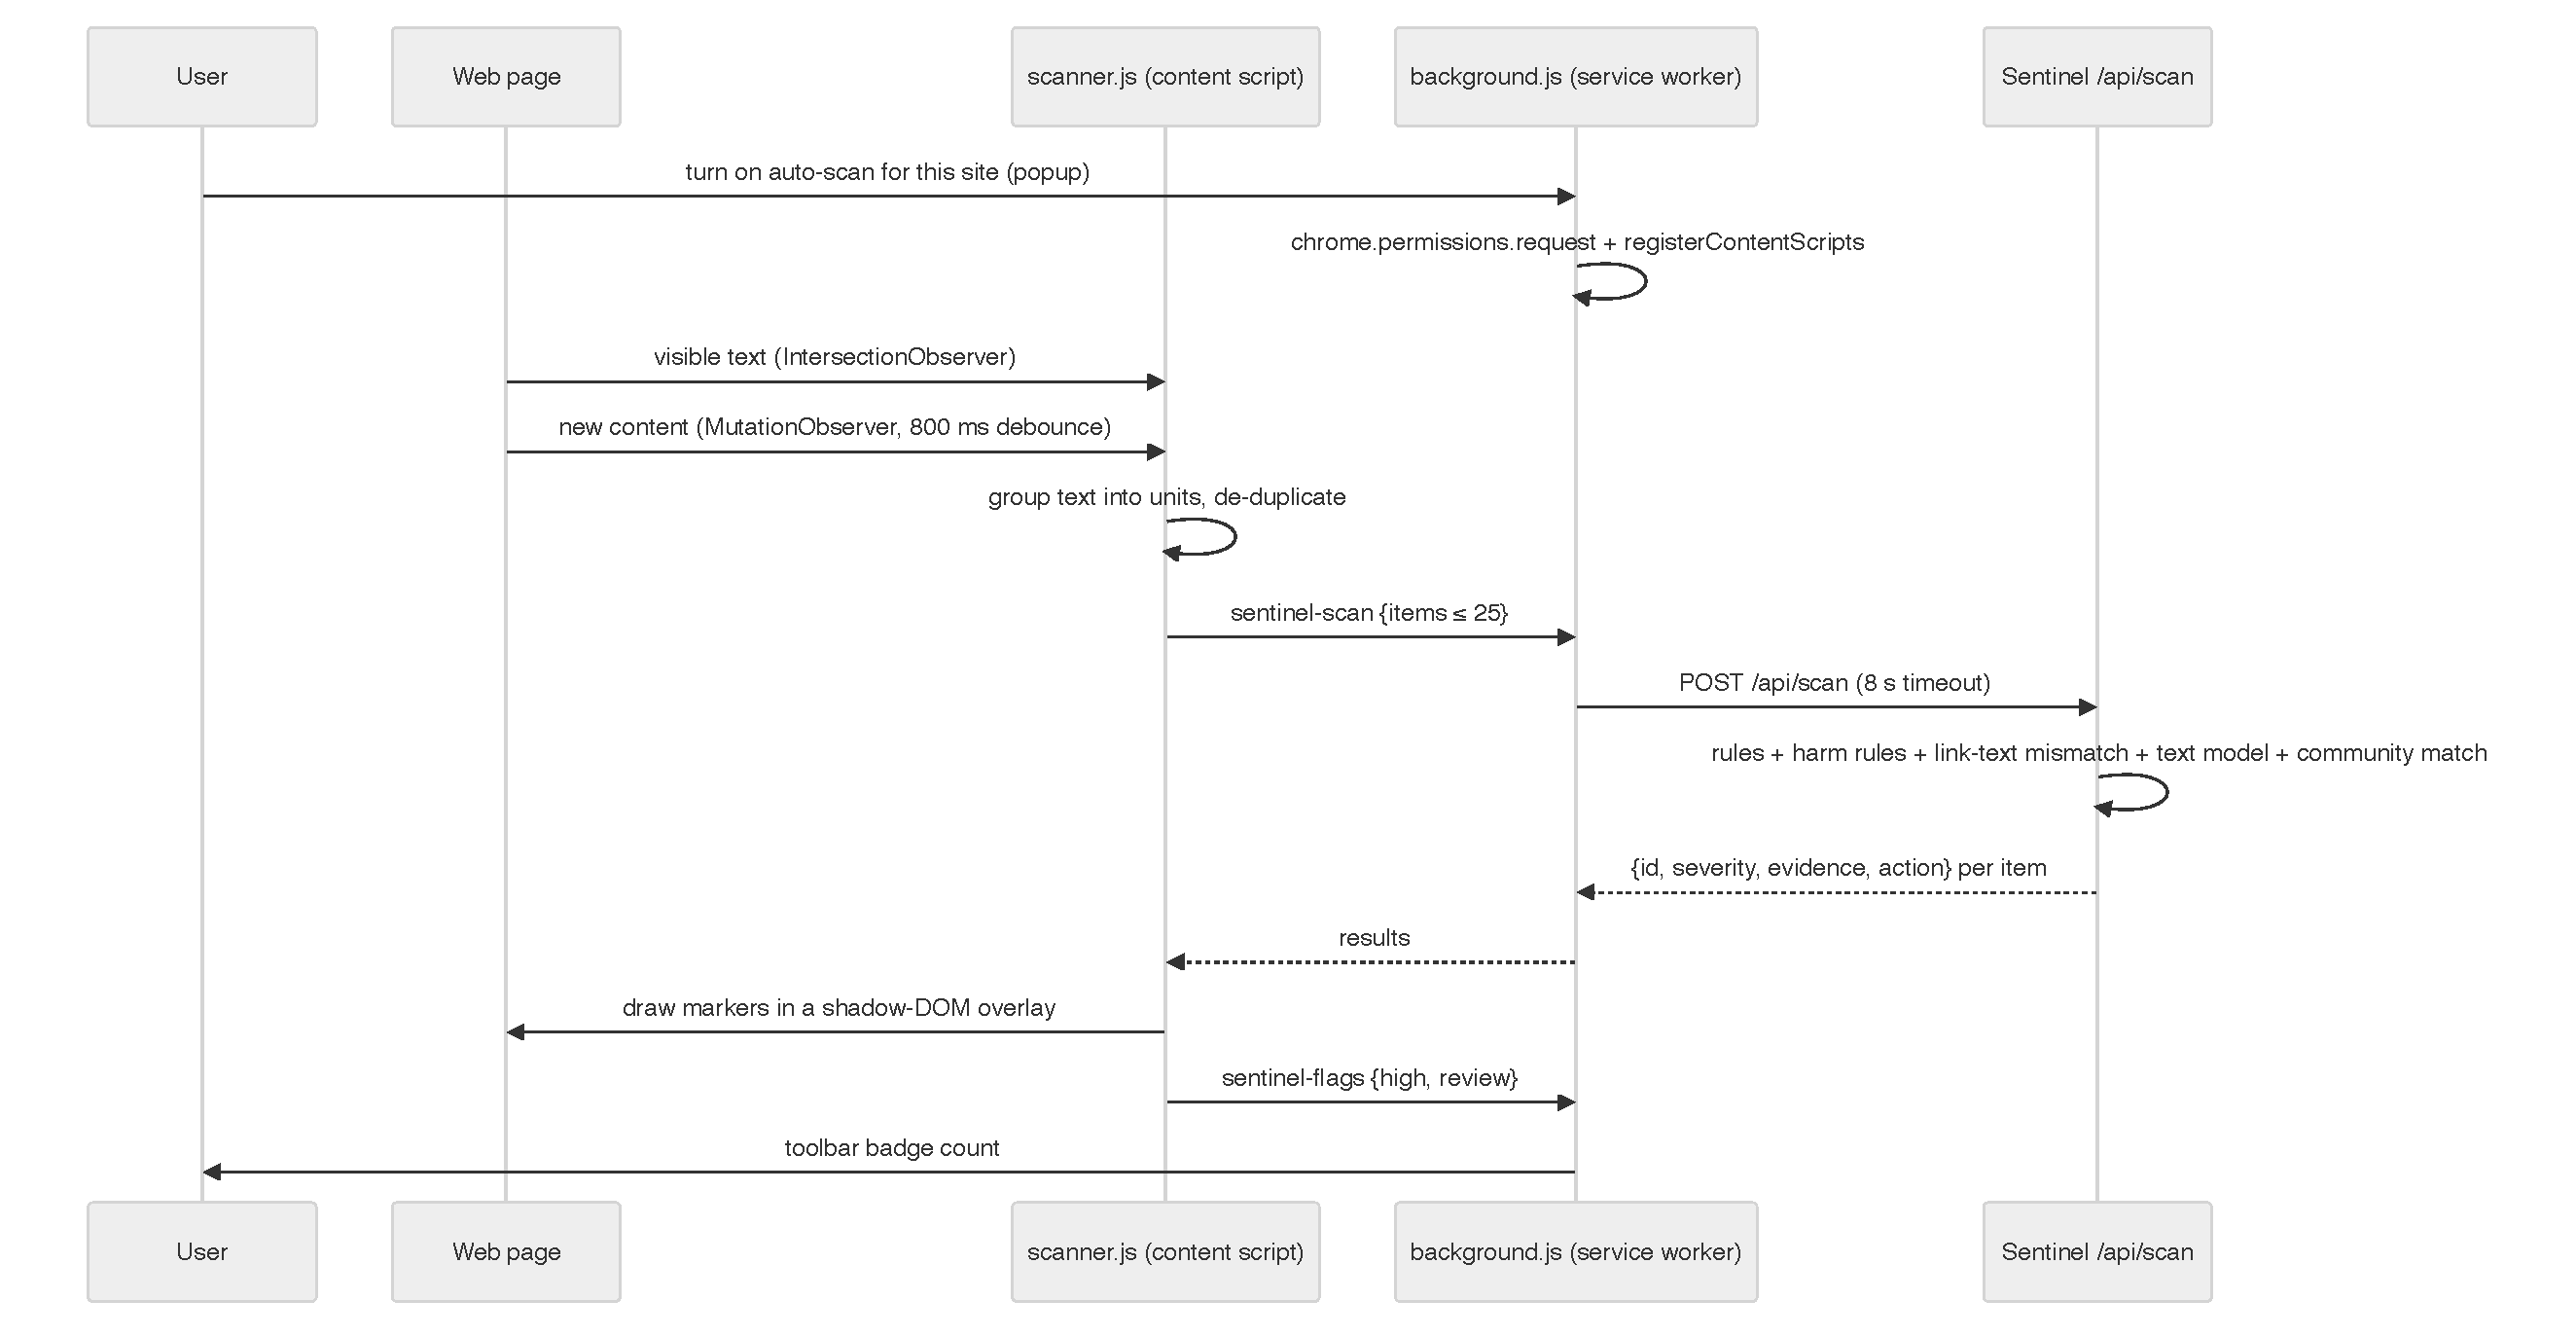
\includegraphics[width=\linewidth]{dia2/autoscan.pdf}
\caption{Sequence diagram: auto-scan of visible page text}
\label{fig:autoscan}
\end{figure}

\subsection{Class Diagram}
\noindent \texttt{create\_server()} creates one \texttt{CaseStore}, one \texttt{SnapshotSigner} and one \texttt{Optional\-Model\-Budget} (which allows one optional model run, reserved at 8 GiB, at a time), shared by every request \texttt{Handler} (aggregation in Figure~\ref{fig:class}). The \texttt{analysis} module creates a \texttt{Conversation\-Input}; the harm service is always present and reports ``unavailable'' without an artifact, while the URL and paired services are created only when configured.
\begin{figure}[H]
\centering
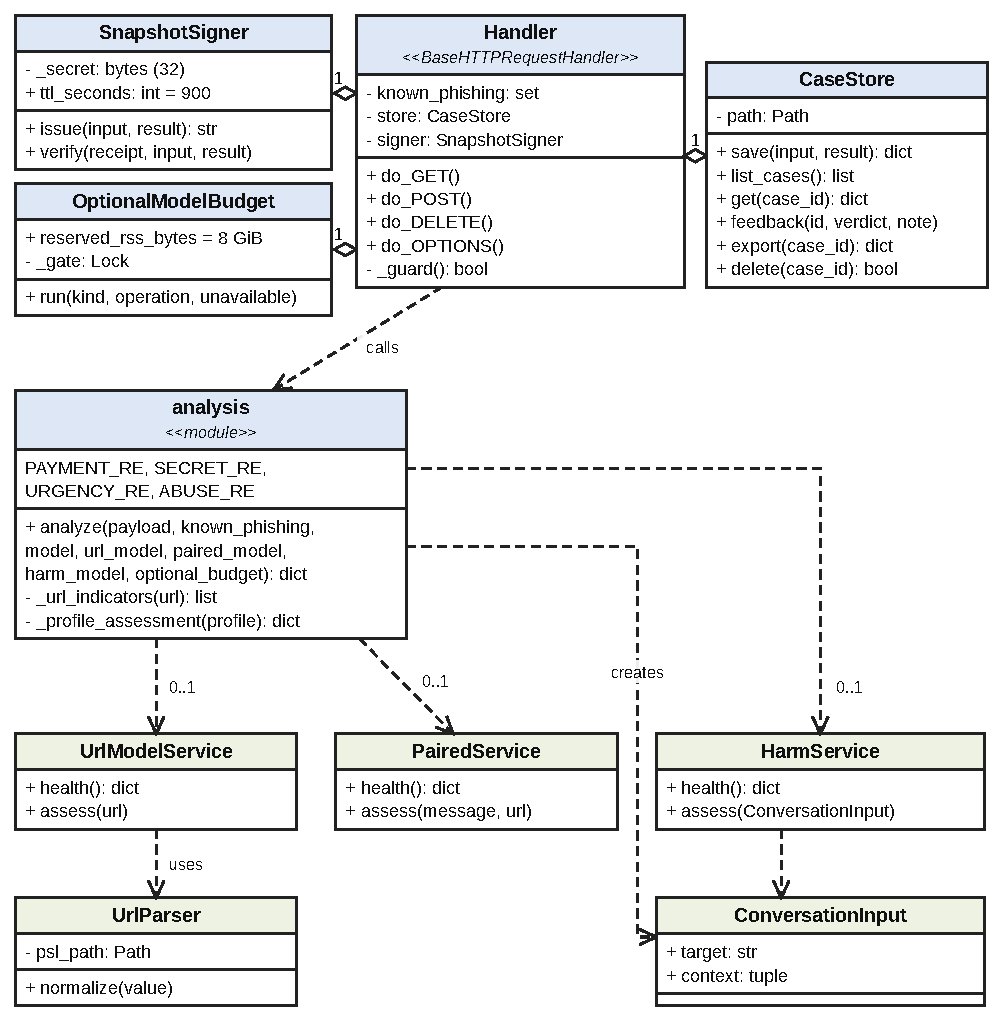
\includegraphics[width=0.9\linewidth]{dia/class.pdf}
\caption{Class diagram of the main application components}
\label{fig:class}
\end{figure}

\subsection{Deployment Diagram}
\noindent The application runs entirely on the user's computer (Figure~\ref{fig:deploy}). Chrome hosts the web client and extension, which send HTTP JSON to the Python process bound to 127.0.0.1:8787, started by \texttt{start-sentinel.sh} with the text-model environment and the model folders. The process loads checksummed model artifacts, writes the SQLite case file and, when configured, talks over loopback to the optional community hub process (127.0.0.1:8790, its own SQLite file) and over HTTPS to fixed official API hosts. The research CLIs run on a research workstation node with the private data, and a checksummed artifact reaches the application only by a manual export.
\begin{figure}[H]
\centering
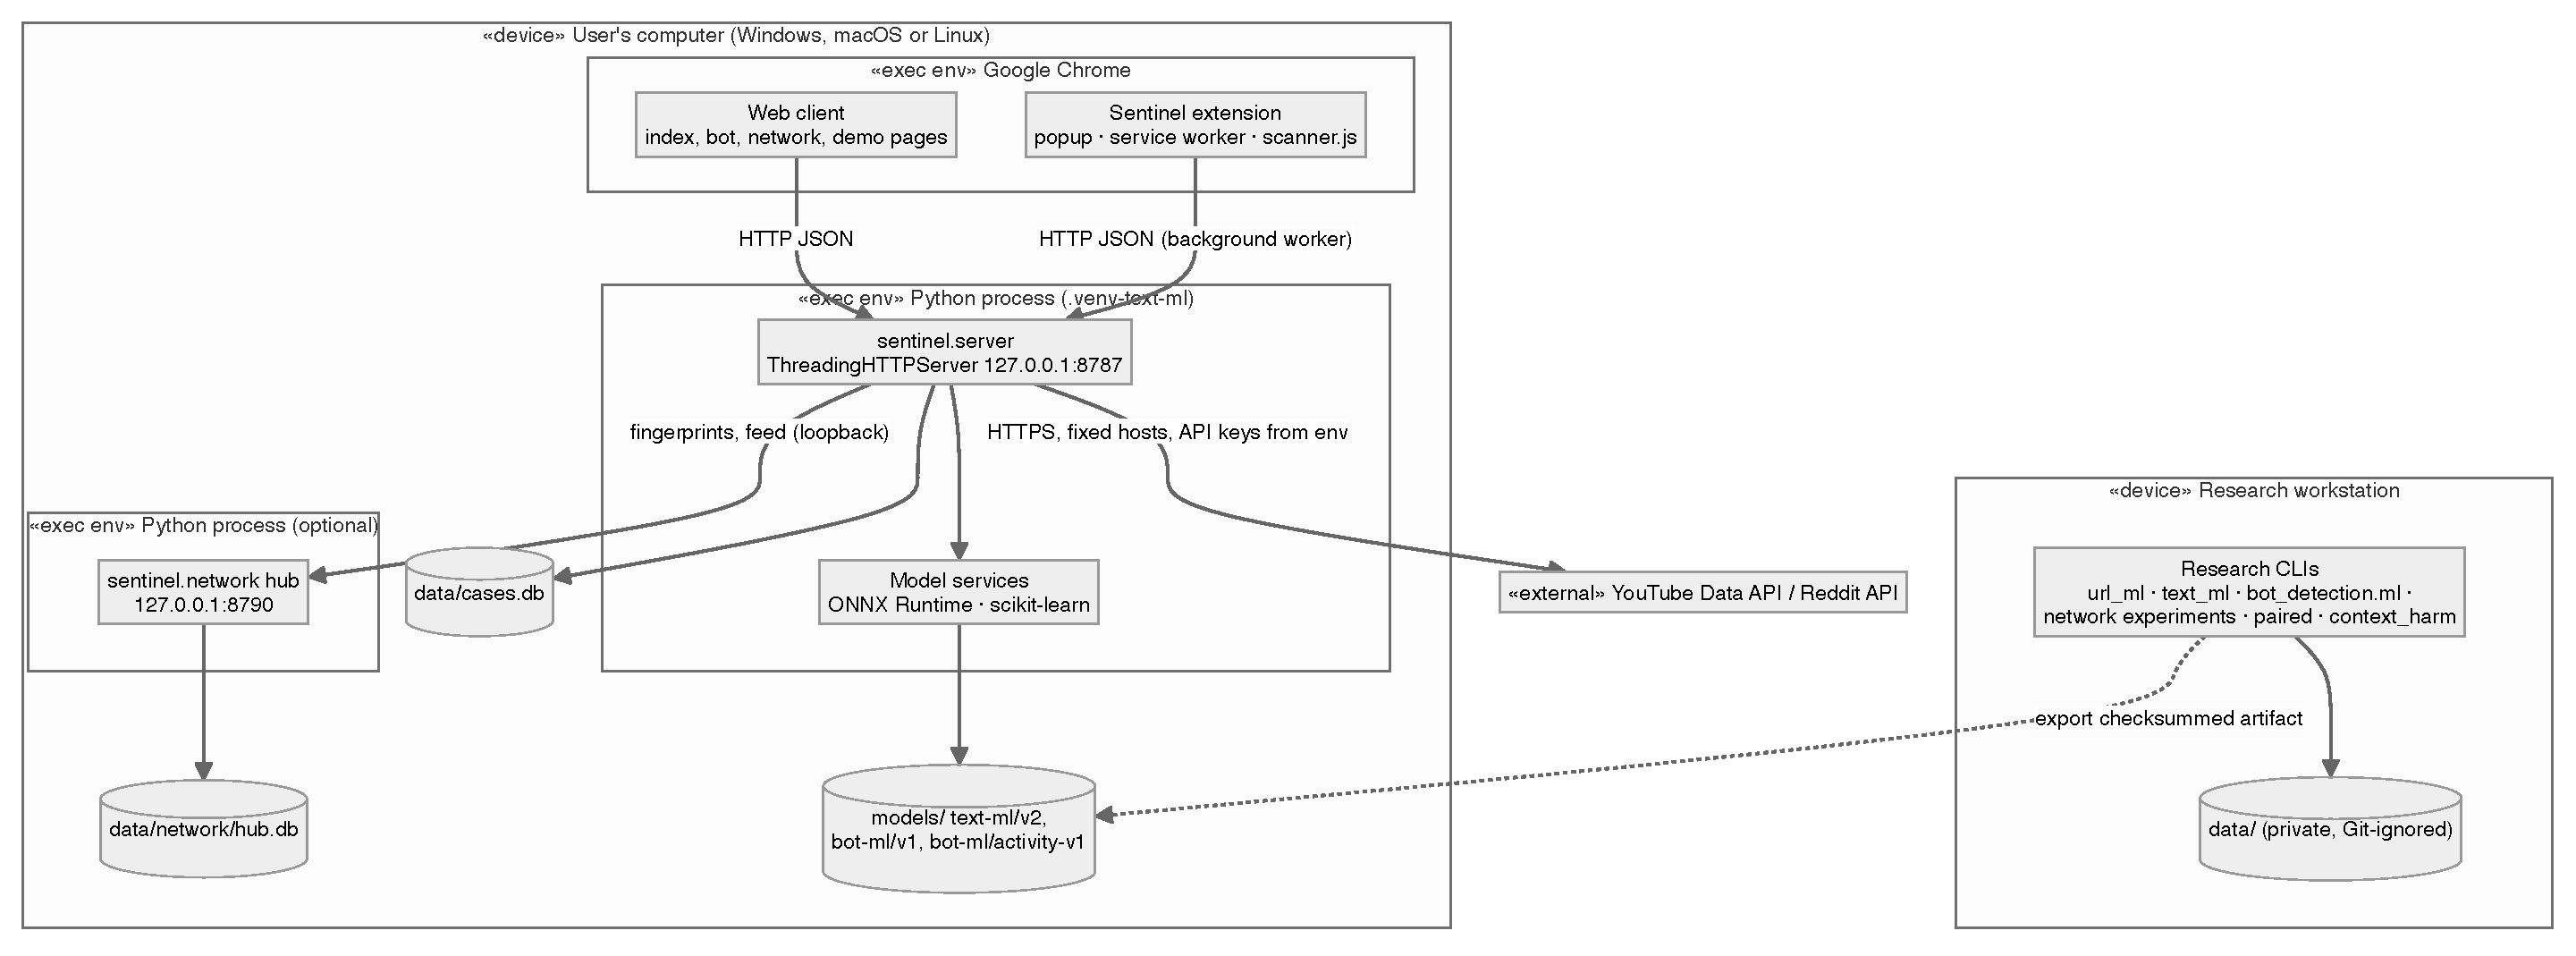
\includegraphics[width=\linewidth]{dia2/deploy_v2.pdf}
\caption{Deployment diagram}
\label{fig:deploy}
\end{figure}

\subsection{ER Diagram and Sample Schema}
\noindent Only cases that the user saves are stored by the application, in one SQLite table; input and result are stored as JSON documents so that the exact reviewed snapshot is preserved (Figure~\ref{fig:er}, Table~\ref{tab:schema}). The USER entity is conceptual (the owner of the device) and is not stored, since the application has no accounts.
\begin{figure}[H]
\centering
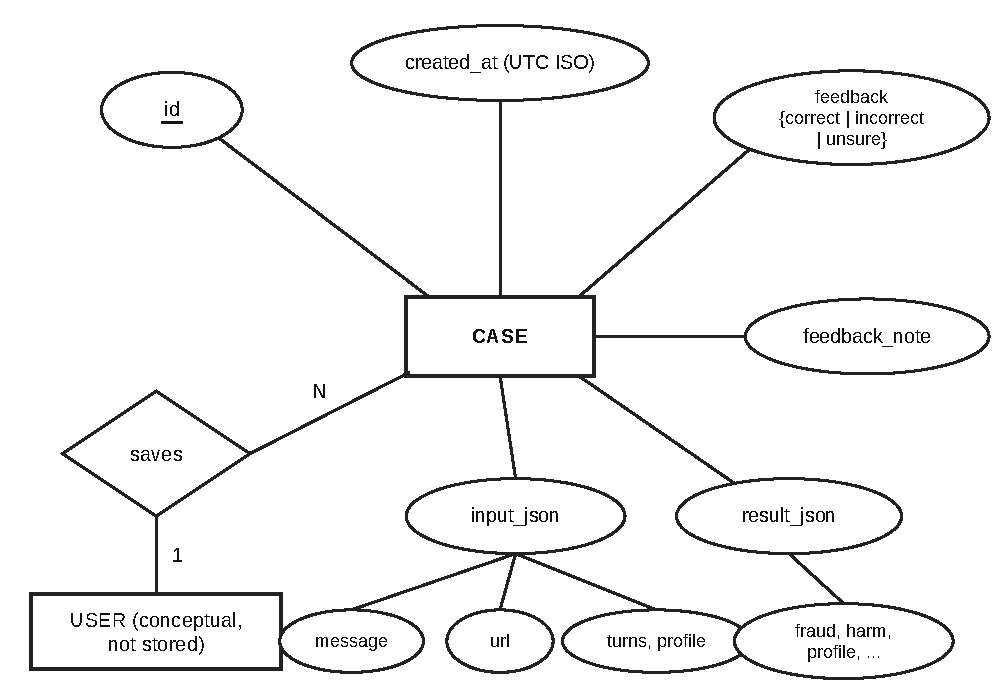
\includegraphics[width=0.8\linewidth]{dia/er.pdf}
\caption{ER diagram of the case store}
\label{fig:er}
\end{figure}

\begin{table}[H]
\centering
\footnotesize
\renewcommand{\arraystretch}{1.2}
\caption{Schema of the \texttt{cases} table with sample values}
\label{tab:schema}
\begin{tabular}{|l|l|l|>{\raggedright\arraybackslash}p{8.2cm}|}
\hline
\textbf{Column} & \textbf{Type} & \textbf{Constraint} & \textbf{Description / sample value} \\ \hline
id & TEXT & PRIMARY KEY & UUID4 hex, e.g. \texttt{3f9c...a1} \\ \hline
created\_at & TEXT & NOT NULL & UTC ISO-8601 time, e.g. \texttt{2026-10-30T15:40:06.123456+00:00} \\ \hline
input\_json & TEXT & NOT NULL & \texttt{\{"message": "You are shortlisted...", "url": "http://192.168.10.5/..."\}} \\ \hline
result\_json & TEXT & NOT NULL & \texttt{\{"fraud": \{"level": "high", ...\}, "harmful\_content": ..., "profile": ...\}} \\ \hline
feedback & TEXT & NULL & correct, incorrect or unsure \\ \hline
feedback\_note & TEXT & NULL & optional note, at most 1,000 characters \\ \hline
\end{tabular}
\end{table}

\noindent The optional community hub keeps its own SQLite database, which holds no message text: \texttt{clients} (random id, creation hour, reputation), \texttt{clusters} (MinHash signature, category, topic tags, salted domain hashes, first and last hour, status, publication hour), \texttt{cluster\_bands} (LSH band key to cluster), \texttt{reports} and \texttt{disputes} (cluster, client, hour, weight), \texttt{attempts} (for rate limiting) and \texttt{allowlist} (verified senders).

\subsection{Data Flow Diagrams}
\noindent At Level 0 (Figure~\ref{fig:dfd0}), Sentinel exchanges content and assessments with the user, receives verified URLs from a feed provider and labelled data from public datasets, and returns metrics and artifacts to the research team.
\begin{figure}[!htbp]
\centering
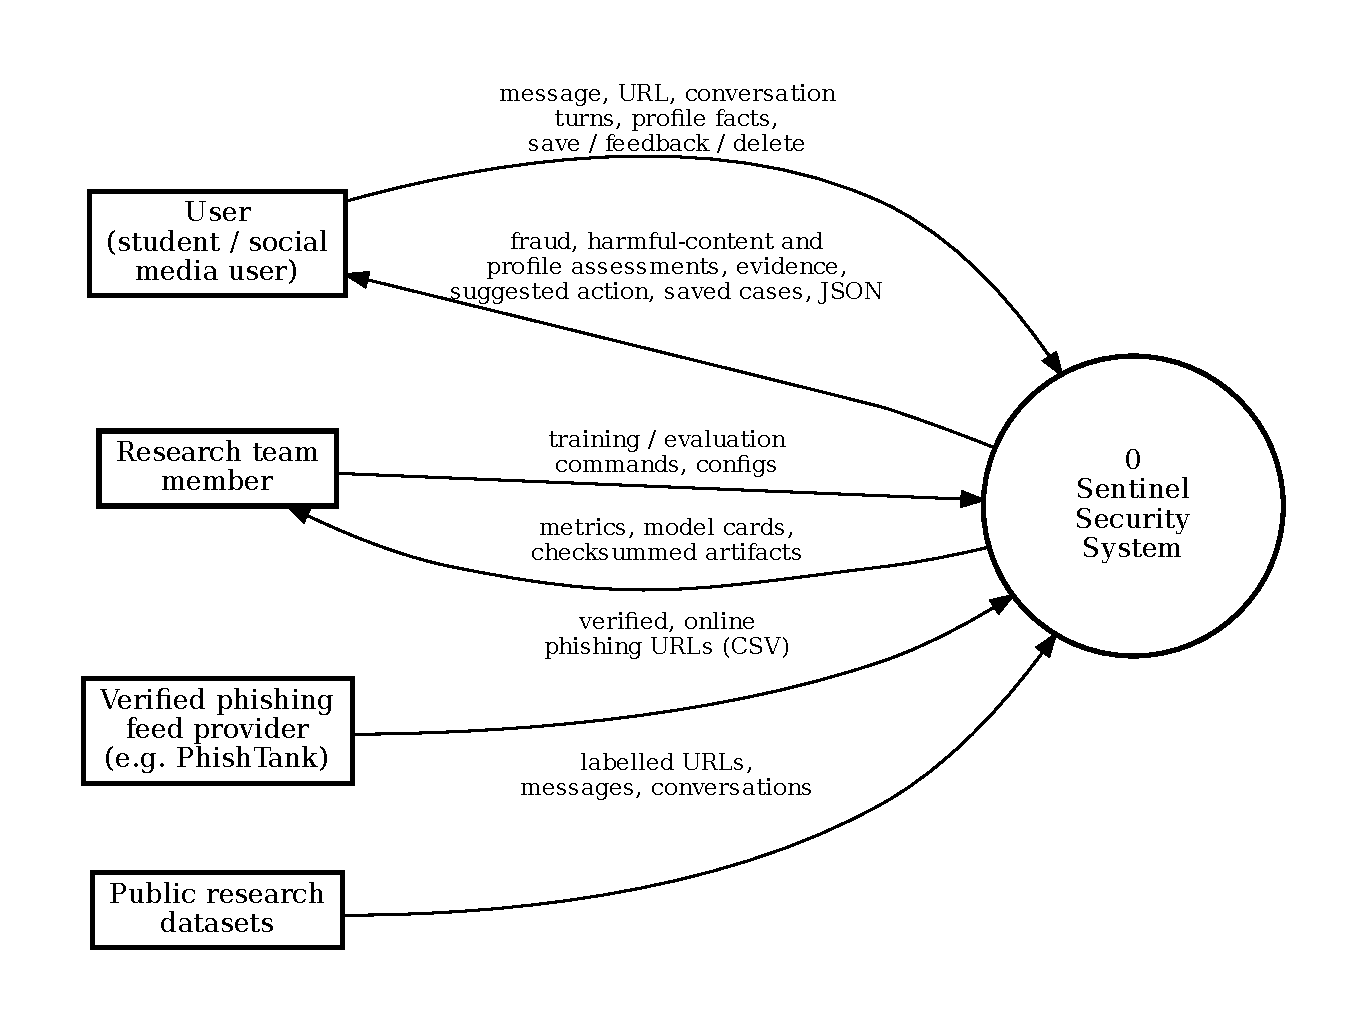
\includegraphics[width=0.84\linewidth]{dia/dfd0.pdf}
\caption{DFD Level 0 (context diagram)}
\label{fig:dfd0}
\end{figure}

\noindent Level 1 (Figure~\ref{fig:dfd1}) decomposes the system into 1.0 Capture input, 2.0 Analyze content, 3.0 Manage saved cases and 4.0 Train and evaluate models, with the data stores D1 case store, D2 phishing feed, D3 model artifacts and D4 private research data. The application side (1.0--3.0) and the research side (4.0) meet only through D3: process 4.0 writes checksummed artifacts that process 2.0 may load as an optional research model.
\begin{figure}[!htbp]
\centering
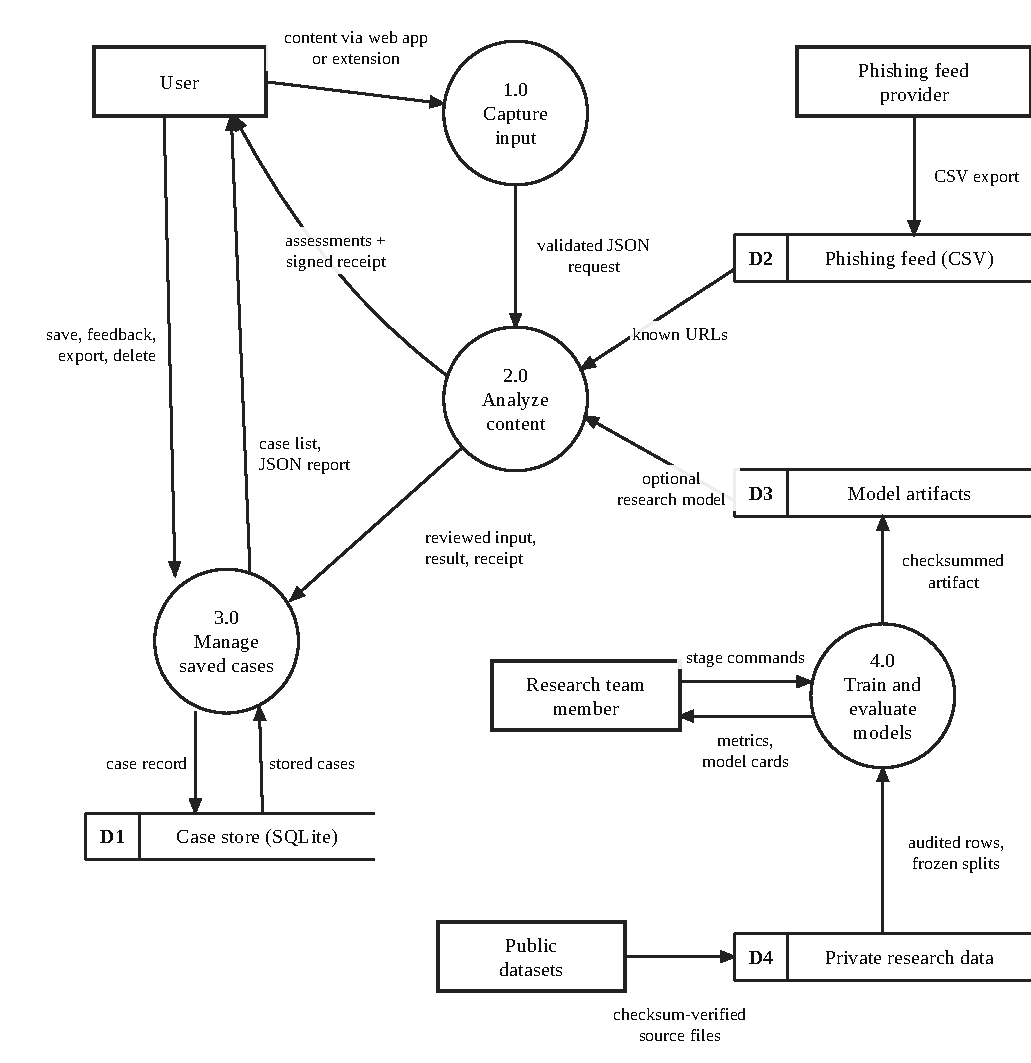
\includegraphics[width=0.86\linewidth]{dia/dfd1.pdf}
\caption{DFD Level 1}
\label{fig:dfd1}
\end{figure}

\noindent Level 2 (Figure~\ref{fig:dfd2a}) expands process 2.0, the core of the application: the request is validated (2.1), the conversation is parsed into a target and its preceding turns (2.2), the URL is extracted (2.3), and the URL-rule and feed lookup (2.5), message rules (2.4), optional research models (2.8), harmful-content check (2.6) and profile indicators (2.7) feed their evidence into result assembly and signing (2.9).
\begin{figure}[!htbp]
\centering
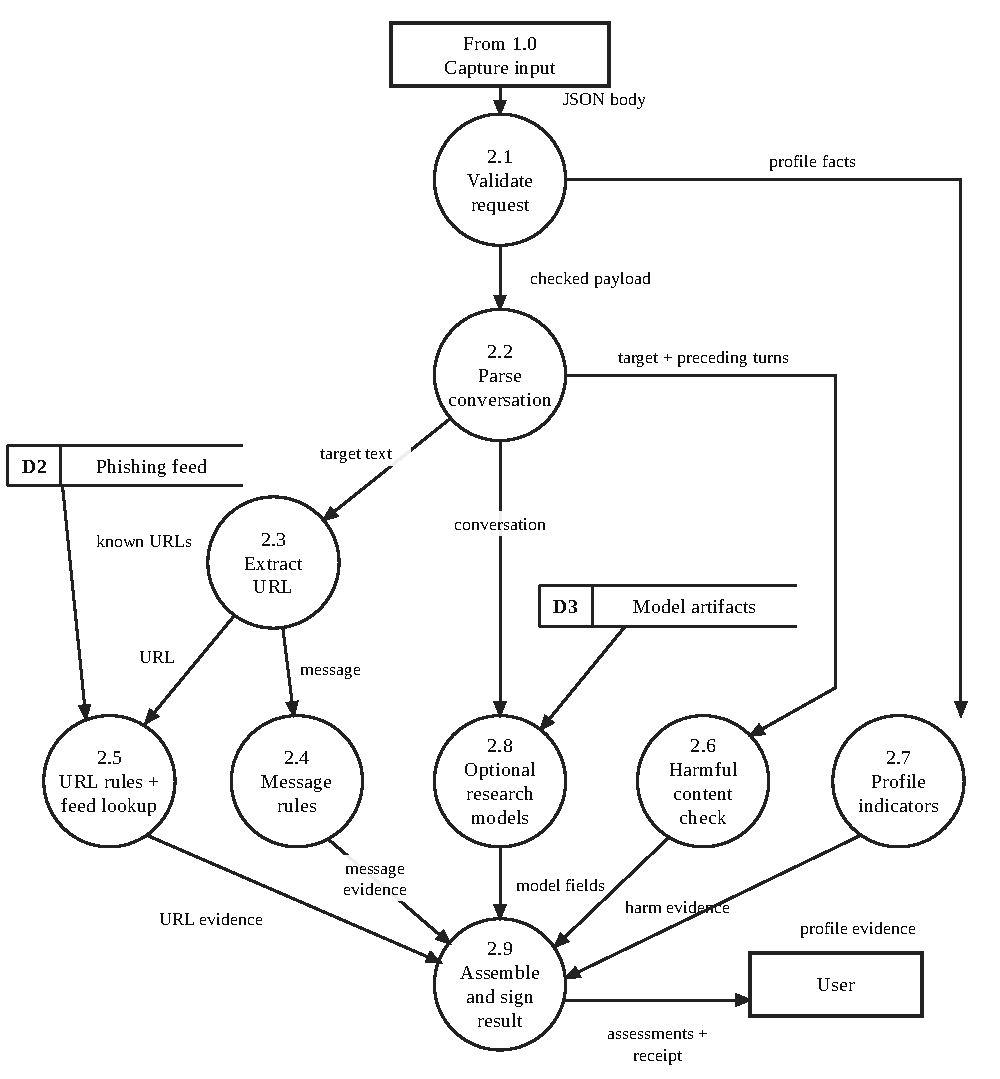
\includegraphics[width=0.86\linewidth]{dia/dfd2a.pdf}
\caption{DFD Level 2 for process 2.0 (Analyze content)}
\label{fig:dfd2a}
\end{figure}

\subsection{Architectural View}
\noindent Sentinel combines four architectural styles. The \textbf{layered style} (Figure~\ref{fig:arch}) has input, preprocessing, detection, analysis and output layers, each using only the one below it, so an analyser can change without changing the interface. The \textbf{client--server style} (Figure~\ref{fig:deploy}) has two thin clients sharing one local server, so both always give the same result for the same input. A \textbf{publish--subscribe style} links clients through the community hub: clients publish fingerprints and poll the campaign feed, without ever talking to each other. The \textbf{pipe-and-filter style} is used by the research pipeline (process 4.0): acquire $\rightarrow$ canonicalise and audit $\rightarrow$ split $\rightarrow$ gate $\rightarrow$ fit $\rightarrow$ select $\rightarrow$ calibrate $\rightarrow$ export $\rightarrow$ evaluate, each filter reading the verified outputs of the previous stage and writing checksummed outputs for the next.

\subsection{Algorithms and Methodology}\label{sec:algos}
\noindent\textbf{Rule patterns} (case-insensitive): \emph{Payment} -- pay, payment, registration/processing fee, send money, UPI; \emph{Secret} -- password, one time password, OTP, verification code, login details; \emph{Urgency} -- act now, immediately, urgent, within $N$ minutes/hours, limited time. The harmful-language rules are described with Algorithm~\ref{alg:harm}. Profile indicators follow M10, and receipts are verified in constant time with a 900-second window and matching SHA-256 hashes of input and result (M11).

\begin{algorithm}[!htbp]
\caption{Fraud (message and link) assessment}\label{alg:fraud}
\begin{algorithmic}[1]
\Require message $m$, supplied URL $u_s$, optional verified feed $F$
\State $u \gets u_s$ if supplied, else the first \texttt{http(s)} link in $m$ (trailing punctuation removed)
\State $E \gets [\,]$; append evidence for each of Payment, Secret, Urgency matched by $m$
\State $U \gets \Call{UrlIndicators}{u}$; \quad $E \gets E \cup U$
\State $known \gets (F \neq \varnothing) \wedge (u \in F)$; if $known$, put ``URL appears in verified feed'' first in $E$
\State $warn \gets m$ matches Payment or Secret
\If{$known \vee (warn \wedge U \neq \varnothing)$} $level \gets$ High
\ElsIf{$E \neq \varnothing$} $level \gets$ Review
\Else\ $level \gets$ Low observed concern
\EndIf
\State add unavailable checks (feed not loaded / URL unlisted / no URL); \Return $level, E$, unavailable checks, uncertainty, action
\end{algorithmic}
\end{algorithm}

\begin{algorithm}[!htbp]
\caption{UrlIndicators($u$)}\label{alg:url}
\begin{algorithmic}[1]
\If{$u$ is empty} \Return $[\,]$ \EndIf
\State parse $u$ into scheme, authority and host (no network access); if parsing fails \Return [``could not be parsed'']
\If{scheme $\notin\{\texttt{http},\texttt{https}\}$ or host is empty} \Return [``incomplete or unexpected scheme''] \EndIf
\State $I \gets [\,]$
\If{``@'' in authority} add ``@ can hide the real host'' \EndIf
\If{host starts with \texttt{xn--} or contains \texttt{.xn--}} add ``punycode domain'' \EndIf
\If{host is an IP address} add ``IP address instead of a named site'' \EndIf
\If{number of dots in host $\ge 4$} add ``long chain of subdomains'' \EndIf
\If{$|u| > 180$} add ``URL is unusually long'' \EndIf
\State \Return $I$
\end{algorithmic}
\end{algorithm}


\noindent\textbf{URL models.} The first branch converts the canonical URL into character 3--5-gram TF-IDF features (at most 50,000), where for an $n$-gram $g$ in URL $d$ among $N$ URLs
\begin{equation}
\mathrm{tfidf}(g,d) = \mathrm{tf}(g,d)\cdot\left(\ln\frac{1+N}{1+\mathrm{df}(g)}+1\right),
\end{equation}
and fits logistic regression with $C\in\{0.1,1,10\}$, with and without class balancing:
\begin{equation}
P(y=1\mid \mathbf{x}) = \sigma(\mathbf{w}^\top\mathbf{x}+b) = \frac{1}{1+e^{-(\mathbf{w}^\top\mathbf{x}+b)}}.
\end{equation}
The second branch computes 16 lexical features (URL, host, path and query lengths; host-label and dot counts; digit, letter and punctuation ratios; hyphen, ``@'' and percent-encoding counts; IP host, punycode, unknown suffix and HTTPS flags) and fits histogram gradient boosting with depth $\in\{3,5\}$ and learning rate $\in\{0.05,0.1\}$.

\begin{algorithm}[!htbp]
\caption{Grouped split allocation (seed 42, target 70/10/10/10)}\label{alg:split}
\begin{algorithmic}[1]
\State group rows by registrable domain using the pinned Public Suffix List
\State shuffle group keys with seed 42, then sort groups by size (largest first)
\ForAll{group $G$ in that order}
  \State assign $G$ to the partition $p$ minimising $\sum_{c\in\{0,1\}} \frac{(n_{p,c}+|G_c|-T_{p,c})^2-(n_{p,c}-T_{p,c})^2}{\max(T_{p,c},1)}$
\EndFor
\State require both classes in every partition; save a SHA-256 manifest of assignments
\end{algorithmic}
\end{algorithm}
\noindent Here $T_{p,c}$ is the target count of class $c$ in partition $p$ and $n_{p,c}$ the count already assigned, so whole domains are placed while class balance stays close to the target.

\begin{algorithm}[!htbp]
\caption{Model selection under a false-positive budget}\label{alg:thresh}
\begin{algorithmic}[1]
\ForAll{configuration $k$ in the grid}
  \State fit on the training partition in a separate process (4 threads, 8 GiB ceiling)
  \State for each distinct validation score $\tau$ compute $\mathrm{FPR}(\tau)$, $\mathrm{Recall}(\tau)$, $\mathrm{Precision}(\tau)$
  \State $\tau_k \gets$ threshold with the highest (recall, precision) such that $\mathrm{FPR}(\tau)\le 0.05$
\EndFor
\State select $k^\ast$ with the best validation recall at $\tau_k$; freeze $\tau_{k^\ast}$
\State fit sigmoid calibration on the calibration partition; score the test partition once
\end{algorithmic}
\end{algorithm}

\noindent\textbf{Calibration.} With raw score $s$ clipped to $[10^{-6},1-10^{-6}]$ and $\mathrm{logit}(s)=\ln\frac{s}{1-s}$,
\begin{equation}
\hat p = \sigma\big(a\cdot\mathrm{logit}(s)+b\big),
\end{equation}
where $a>0$ and $b$ are fitted by logistic regression on the calibration partition only. Calibration is reported as unavailable if there are fewer than 100 rows or 20 per class, if the score logits do not vary, if the fit fails, or if the slope is not positive.\\

\noindent\textbf{Paired message--link baseline.} Multinomial Naive Bayes with Laplace smoothing over message tokens (URL spans removed), URL host/path tokens with structural flags, or both:
\begin{equation}
\hat y = \arg\max_{c\in\{0,1\}}\Big[\ln P(c)+\sum_{t} n_t \ln\frac{\mathrm{count}(t,c)+1}{\sum_{t'}\mathrm{count}(t',c)+|V|}\Big].
\end{equation}
Rows sharing a destination domain, campaign or normalised wording are kept on the same side of the split. The full paired study adds a message branch (word 1--2-gram TF-IDF with logistic regression), a URL branch (lexical features with gradient boosting), early fusion and out-of-fold late fusion.\\

\noindent\textbf{Contextual directed abuse.} A target-only and a context-aware model (word 1--2-gram TF-IDF with logistic regression, $C\in\{0.5,1,2\}$, up to four preceding turns, at most 30,000 target features, plus 30,000 context features in the context-aware model) are compared, with a conditional DistilBERT encoder (sequence length 256, learning rate $2\times10^{-5}$ or $5\times10^{-5}$, at most 3 epochs, bounded to 3.2 GiB of GPU memory). All authors of published test threads are reserved, and training requires at least 200 positive cases and at least ten independent components in validation and calibration.

\begin{algorithm}[!htbp]
\caption{Harmful-language assessment}\label{alg:harm}
\begin{algorithmic}[1]
\Require text $x$ (target message plus conversation context)
\If{$x$ is empty} \Return Not assessed \EndIf
\State $c \gets \Call{Normalise}{x}$: NFKC; look-alike letters mapped; dotted letters joined (\texttt{k.y.s}$\to$\texttt{kys}); leetspeak mapped inside words only; runs of a repeated letter collapsed
\State $I \gets$ spans of known idioms in $c$ (``killed it'', ``shoot me an email'', ``kill the process'', \dots)
\State $reported \gets x$ contains quoted or reported speech
\ForAll{rule $(category, severity, pattern)$ of the 19 rules}
  \State $m \gets$ first match of $pattern$ in $c$ outside $I$; \textbf{if} none \textbf{continue}
  \State $neg \gets$ a negation occurs within 40 characters before $m$ (not for self-harm risk)
  \If{$severity=$ high $\wedge$ ($neg$ $\vee$ ($reported \wedge category \neq$ self-harm risk))} $severity \gets$ review
  \ElsIf{$severity=$ review $\wedge$ $neg$} \textbf{continue}
  \EndIf
  \State record $(category, severity)$ with its description as evidence
\EndFor
\State $level \gets$ High if any match is high, else Review if any is review, else Low observed concern
\State $action \gets$ advice of the most urgent category in the fixed priority (self-harm risk, mass violence, threats, sextortion, blackmail, self-harm encouragement, doxxing, hate, harassment)
\State \Return $level$, categories, evidence, uncertainty, $action$
\end{algorithmic}
\end{algorithm}

\noindent\textbf{Scam-text model.} For a message with DistilBERT logits $\mathbf{z}$ over (ham, spam, smishing), temperature scaling gives $\mathbf{p}^{\mathrm{T}}=\mathrm{softmax}(\mathbf{z}/T)$, with $T=1.2916$ fitted on the calibration split by minimising the negative log-likelihood $-\frac1n\sum_i\ln p_{y_i}$ (golden-section search on $[0.05,10]$) \cite{guo}. The TF-IDF model gives $\mathbf{p}^{\mathrm{L}}$, and the ensemble and scam score are
\begin{equation}
\mathbf{p}=\tfrac12\big(\mathbf{p}^{\mathrm{T}}+\mathbf{p}^{\mathrm{L}}\big),\qquad s = p_{\mathrm{spam}}+p_{\mathrm{smishing}},\qquad \text{flag if } s\ge\tau=0.6108 .
\end{equation}
Training uses class-weighted cross-entropy with $w_c=\sqrt{N/(3N_c)}$, AdamW at learning rate $3\times10^{-5}$, batch 32, maximum length 128 and 4 epochs. The threshold $\tau$ is the one with the best calibration-split recall among those keeping the ham false-positive rate at or below 1\%, the highest such threshold on ties, capped at 0.9, computed on the ONNX outputs the application serves. The ensemble was chosen among three candidates (transformer, TF-IDF, average) by a rule fixed in advance: the highest calibration macro-F1 with calibration ham FPR $\le$ 1\%. A flag is explained by occlusion: the influence of word $w_i$ is
\begin{equation}
\Delta_i=\mathrm{logit}(s)-\mathrm{logit}(s_{-i}),\qquad \mathrm{logit}(s)=\ln\frac{s}{1-s},
\end{equation}
where $s_{-i}$ is the score with $w_i$ removed; log-odds are used because probabilities saturate near 1.

\begin{algorithm}[!htbp]
\caption{Auto-scan severity for one page item}\label{alg:scan}
\begin{algorithmic}[1]
\Require item text and optional link; fraud result $F$, harm result $H$, text-model result $M$, link-text mismatch $L$, community match $C$
\If{$F=$ High $\vee$ $H=$ High $\vee$ ($L \wedge F$ has evidence) $\vee$ ($M$ flagged $\wedge$ ($F$ has evidence $\vee\, L \,\vee\, s\ge0.9$))} $sev\gets$ high
\ElsIf{$M$ flagged $\vee\, L \,\vee\, H=$ Review $\vee$ $F$ has $\ge 2$ pieces of evidence} $sev\gets$ review
\Else\ $sev\gets$ none \Comment{a single weak indicator is too common to mark}
\EndIf
\If{$C$ matched} raise none to review, or review to high when $M$, $F$ or $L$ also found something \EndIf
\State \Return $sev$, evidence, action
\end{algorithmic}
\end{algorithm}

\noindent\textbf{Community fingerprints and publishing.} The masked template is split into word 3-grams $A$. With 64 hash functions $h_j(x)=(a_jx+b_j)\bmod(2^{61}-1)$, the MinHash signature is $\mathrm{sig}_j(A)=\min_{x\in A}h_j(x)$, and for two messages $\Pr[\mathrm{sig}_j(A)=\mathrm{sig}_j(B)]=J(A,B)=|A\cap B|/|A\cup B|$ \cite{broder}. The signature is cut into $b=32$ bands of $r=2$ rows, so two messages of similarity $J$ share at least one band key with probability
\begin{equation}
P(J)=1-\big(1-J^{\,r}\big)^{b},
\end{equation}
which is about 0.997 at $J=0.41$ (16 bands of 4 rows would give only about 0.37) \cite{mmds}. Reports whose estimated similarity is at least 0.4 join a cluster. A cluster is published when it has at least $k=5$ distinct reporters and total weight $\sum_i w_i\ge5$, where a client's weight is 0.5 during its first 24 hours and grows with reputation \cite{sweeney}; it is held for review if it matches the verified-sender allowlist, and withdrawn when disputes reach $\max(k,\,0.5\times\text{reports})$. A published campaign's confidence decays with a 24-hour half-life, $\mathrm{conf}=\sum_i w_i\,0.5^{(t-t_i)/24}$. Figure~\ref{fig:network} summarises the flow.
\begin{figure}[H]
\centering
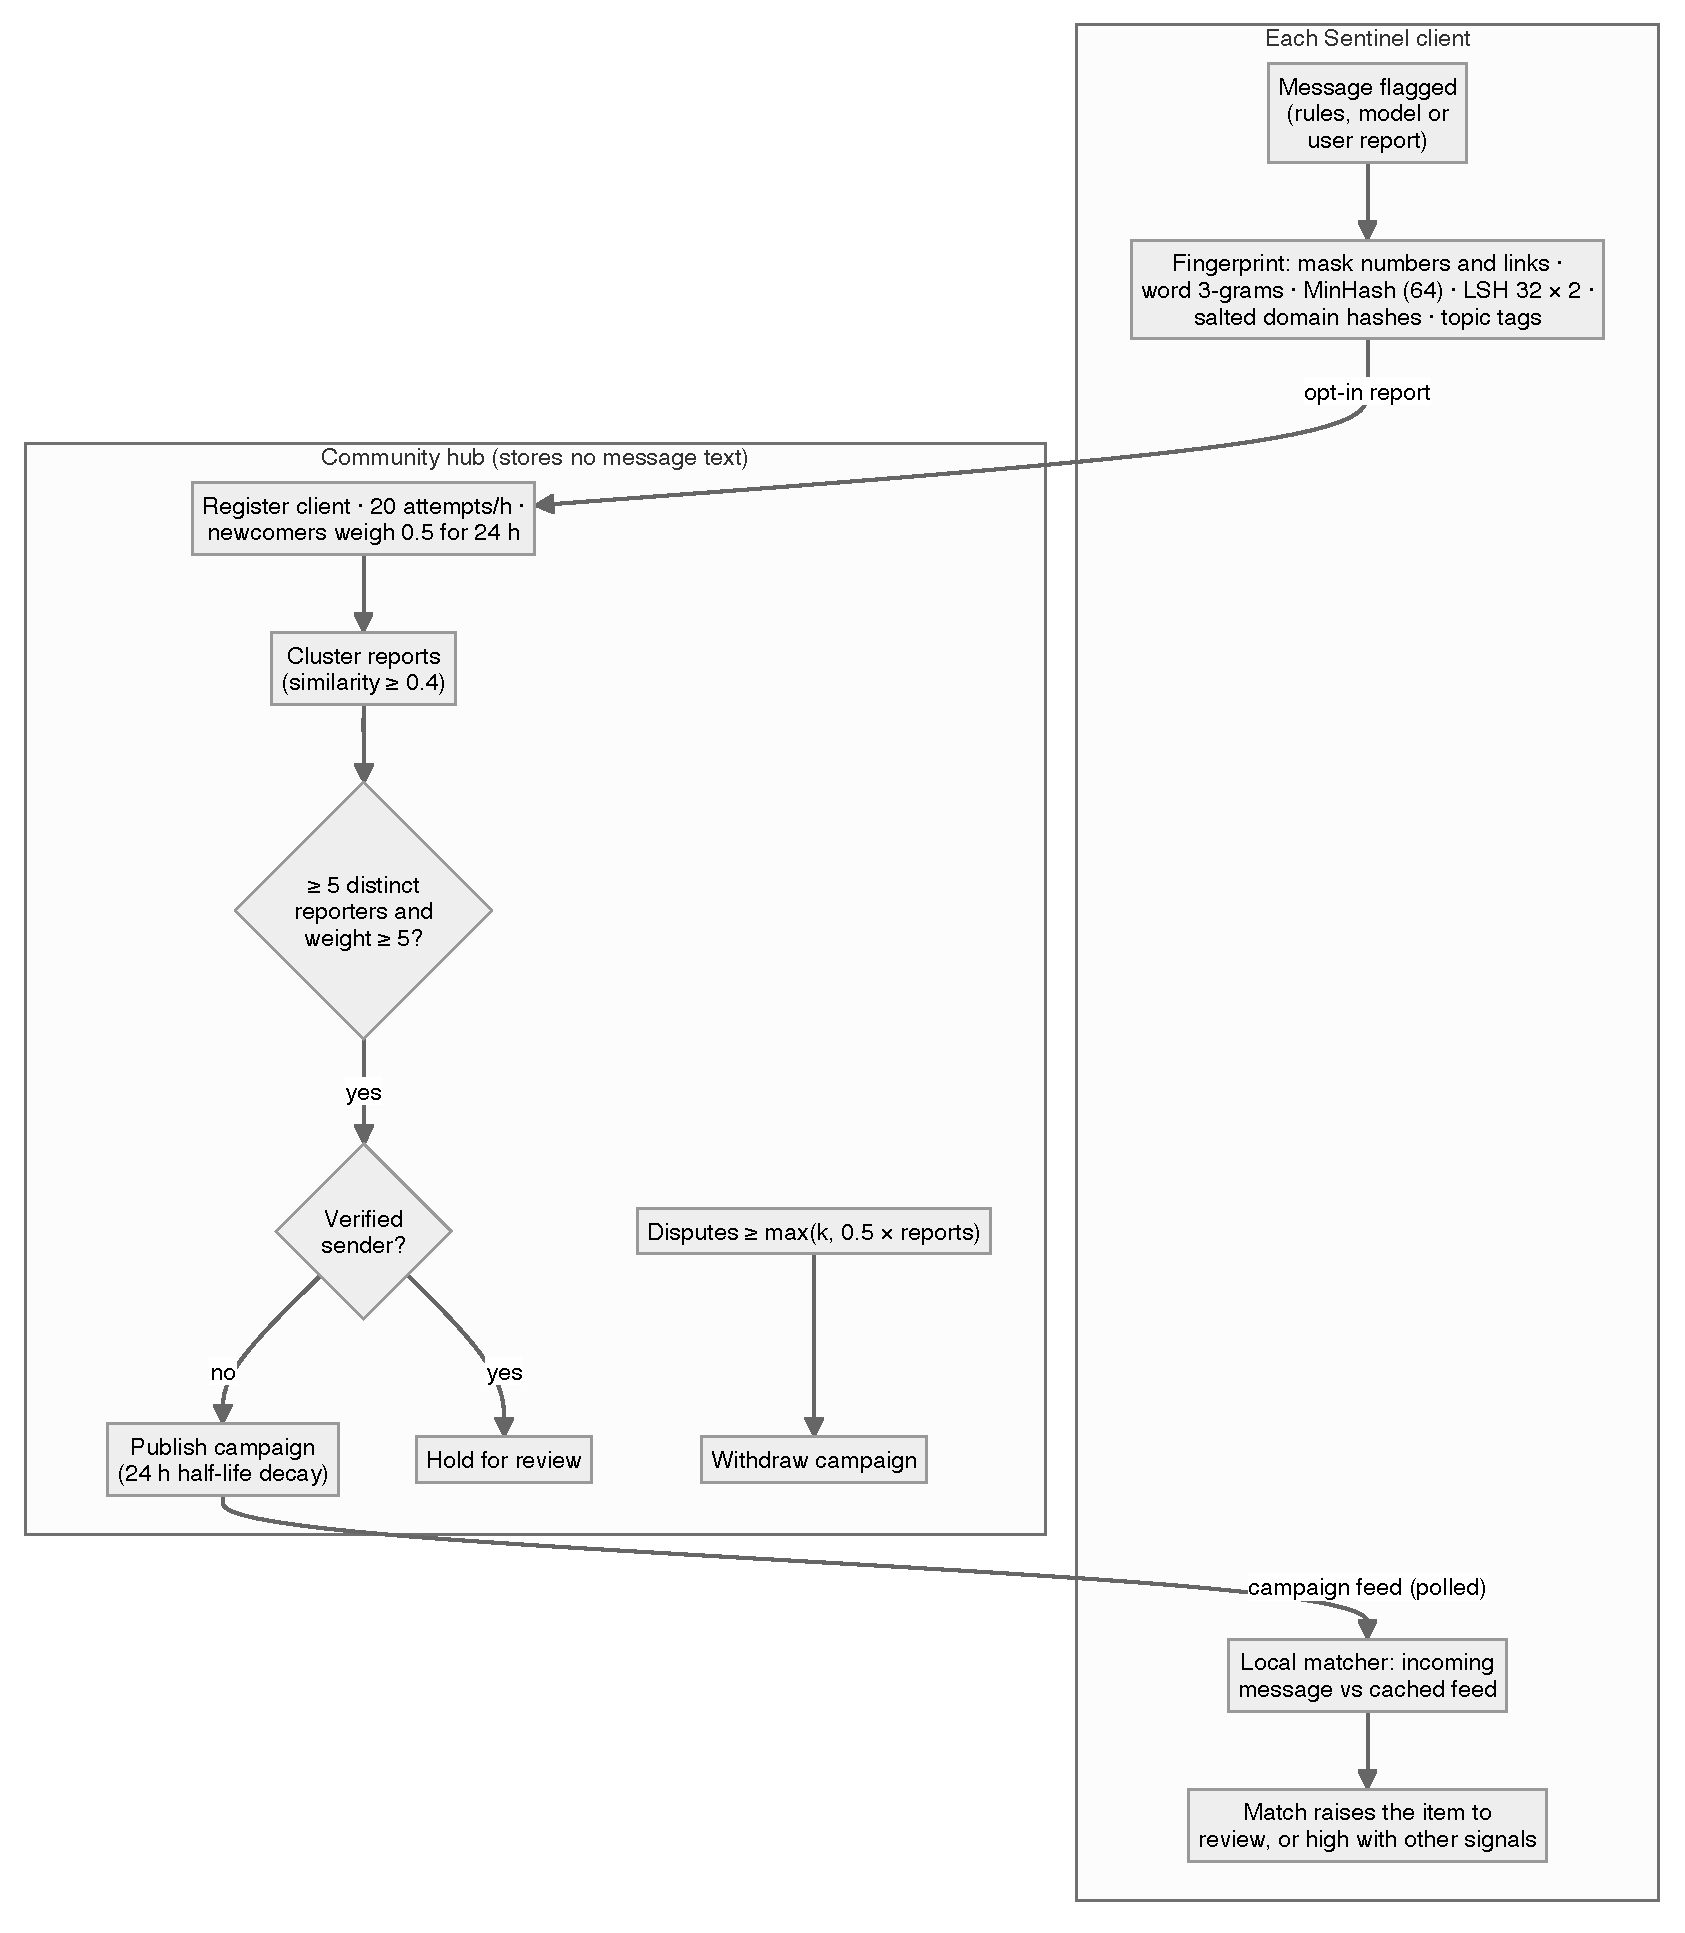
\includegraphics[width=0.74\linewidth]{dia2/network.pdf}
\caption{Community scam network: fingerprinting, publishing and local matching}
\label{fig:network}
\end{figure}

\noindent\textbf{Bot-detection score.} Each of the 25 signals $i$ with data maps a feature to a suspicion $s_i\in[0,1]$ by a linear ramp between two thresholds and has a weight $w_i$ (\texttt{weights.json}). The heuristic score and coverage are
\begin{equation}
\text{score}=100\cdot\frac{\sum_{i\in A} w_i s_i}{\sum_{i\in A} w_i},\qquad \text{coverage}=\frac{\sum_{i\in A}w_i}{\sum_{i}w_i},
\end{equation}
where $A$ is the set of signals that had data. Confidence is High with coverage $\ge 0.65$ and at least 50 posts, Medium with $\ge 0.4$ and 20 posts, and Very low below 0.25 coverage or 4 signals, when the score is withheld. Example activity features are the coefficient of variation of the gaps between posts, $\mathrm{CV}=\sigma/\mu$ (scheduled bots are near 0), the normalised hour-of-day entropy $H=-\sum_h p_h\log_2p_h/\log_2 24$, and the share of near-duplicate posts (MinHash similarity $\ge 0.8$). The trained models are histogram gradient boosting or logistic regression \cite{sklearn} calibrated by isotonic regression \cite{zadrozny}, and are evaluated by leaving out whole datasets or bot families \cite{yang2020}. Figure~\ref{fig:bot} shows the pipeline.
\begin{figure}[H]
\centering
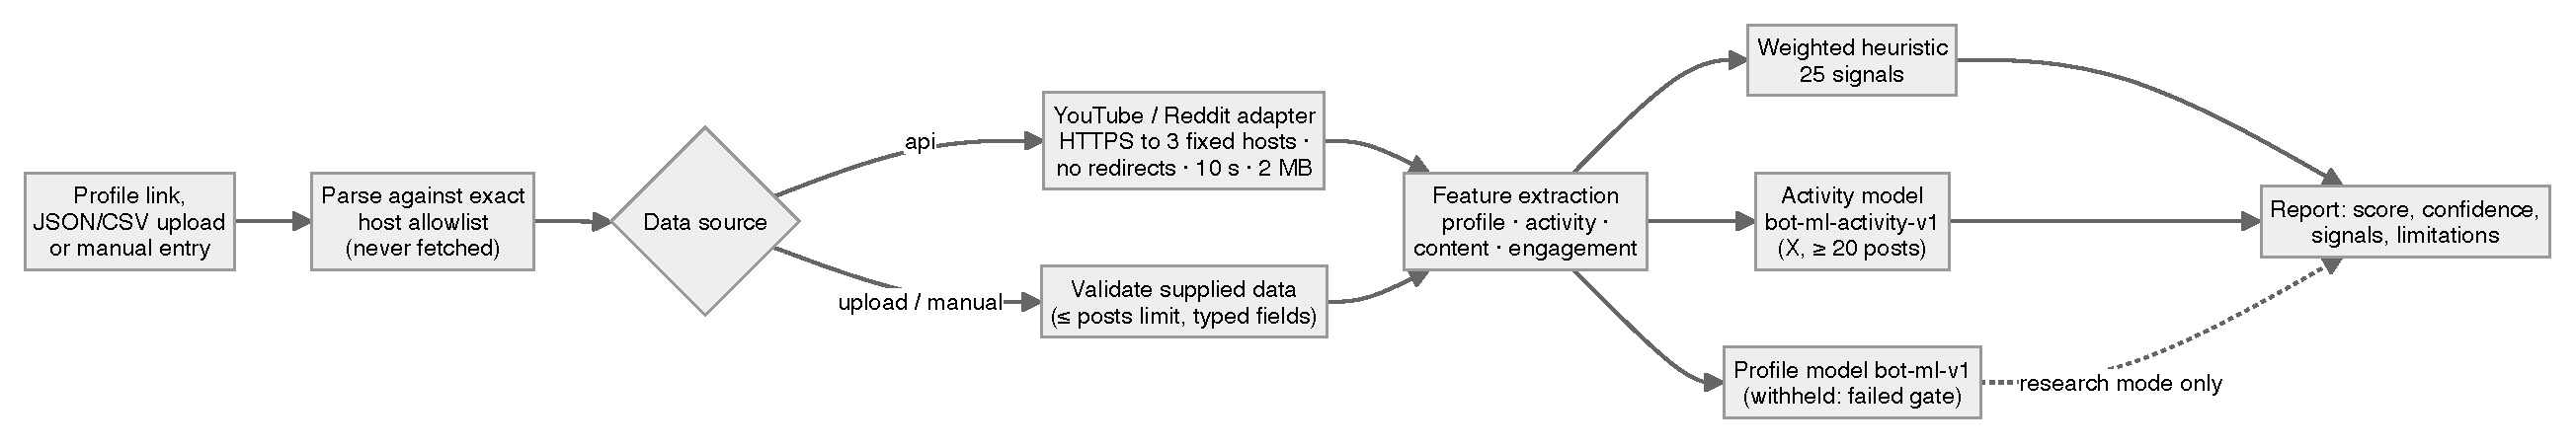
\includegraphics[width=\linewidth]{dia2/bot.pdf}
\caption{Bot-account detection pipeline}
\label{fig:bot}
\end{figure}

\FloatBarrier
\subsection{UI/UX Design}
\noindent The interface follows four principles: plain language, separation of the threat types, honesty about limits and no surprise storage. All pages share one navigation bar (Check content, Bot accounts, Community network, Auto-scan demo, Saved cases). The check form (Figure~\ref{fig:ui-form}a) places the input on the left and the assessments on the right so they can be compared; an overall summary ring counts how many analysers raised concern. Each assessment is a card with a level badge that carries a text label as well as colour, a list of observations, ``Could not check'' lines, an uncertainty sentence and a bold next step; the learned-model card underlines the words that raised the scam score. The extension popup (Figure~\ref{fig:ui-form}b) gives the same cards in a narrow layout; the current popup also has an auto-scan switch for the open site, which this earlier screenshot predates. The Bot accounts page (Figure~\ref{fig:ui-more}a) shows a score gauge, confidence, coverage and the signals behind the score, and the Community network page (Figure~\ref{fig:ui-more}b) shows the hub's live campaigns and what the hub stores. Results are announced to screen readers through an \texttt{aria-live} region, and submitted text is always inserted as text, never as HTML.
\begin{figure}[!htbp]
\centering
\begin{minipage}[b]{0.66\linewidth}\centering
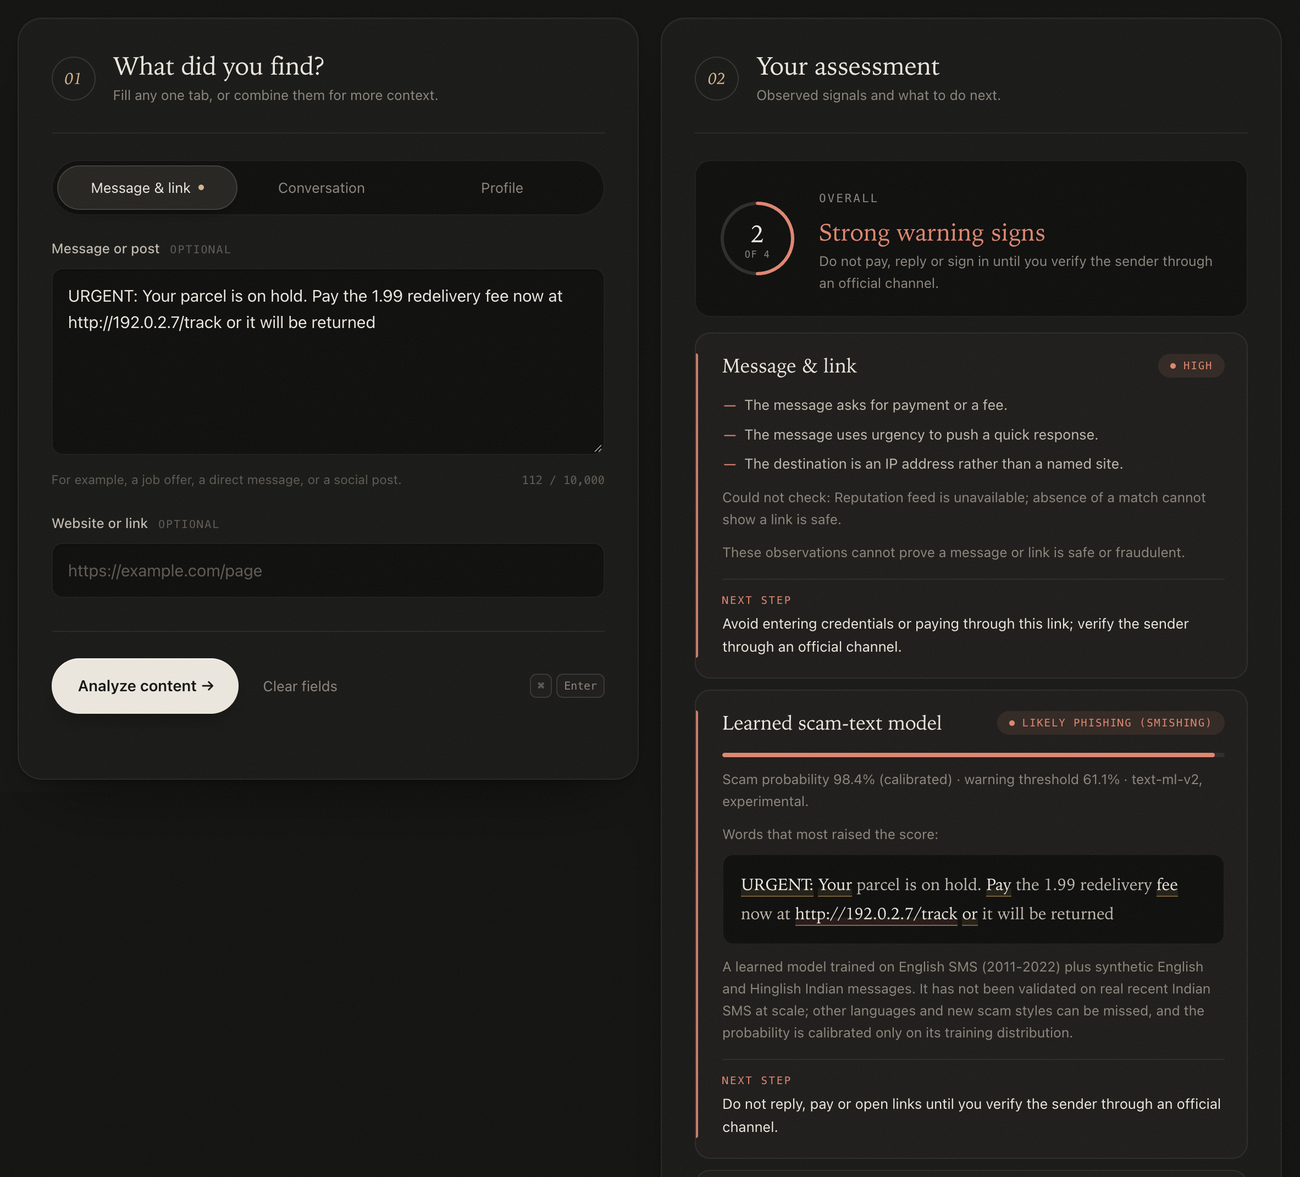
\includegraphics[width=\linewidth]{shots2/check_scam.png}\\[1pt]{\small (a) Web app: check form and assessments for a parcel-fee scam (TC-24)}
\end{minipage}\hfill
\begin{minipage}[b]{0.29\linewidth}\centering
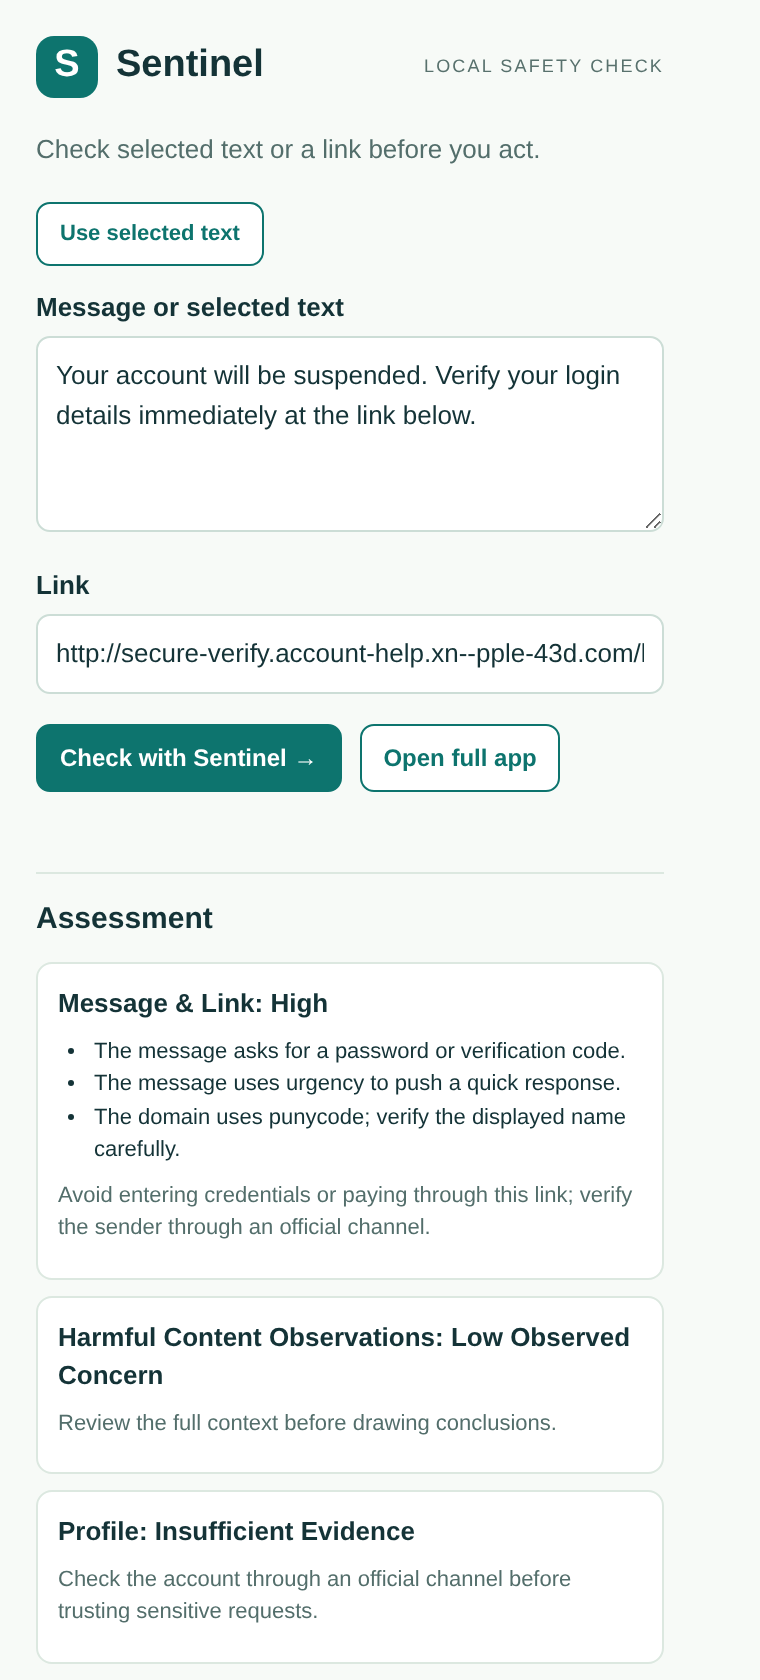
\includegraphics[width=\linewidth]{shots/13_popup_crop.png}\\[1pt]{\small (b) Extension popup}
\end{minipage}
\caption{User interface of Sentinel (popup rendered from its own code against the local API; lower cards cropped)}
\label{fig:ui-form}
\end{figure}

\begin{figure}[!htbp]
\centering
\begin{minipage}[t]{0.40\linewidth}\centering
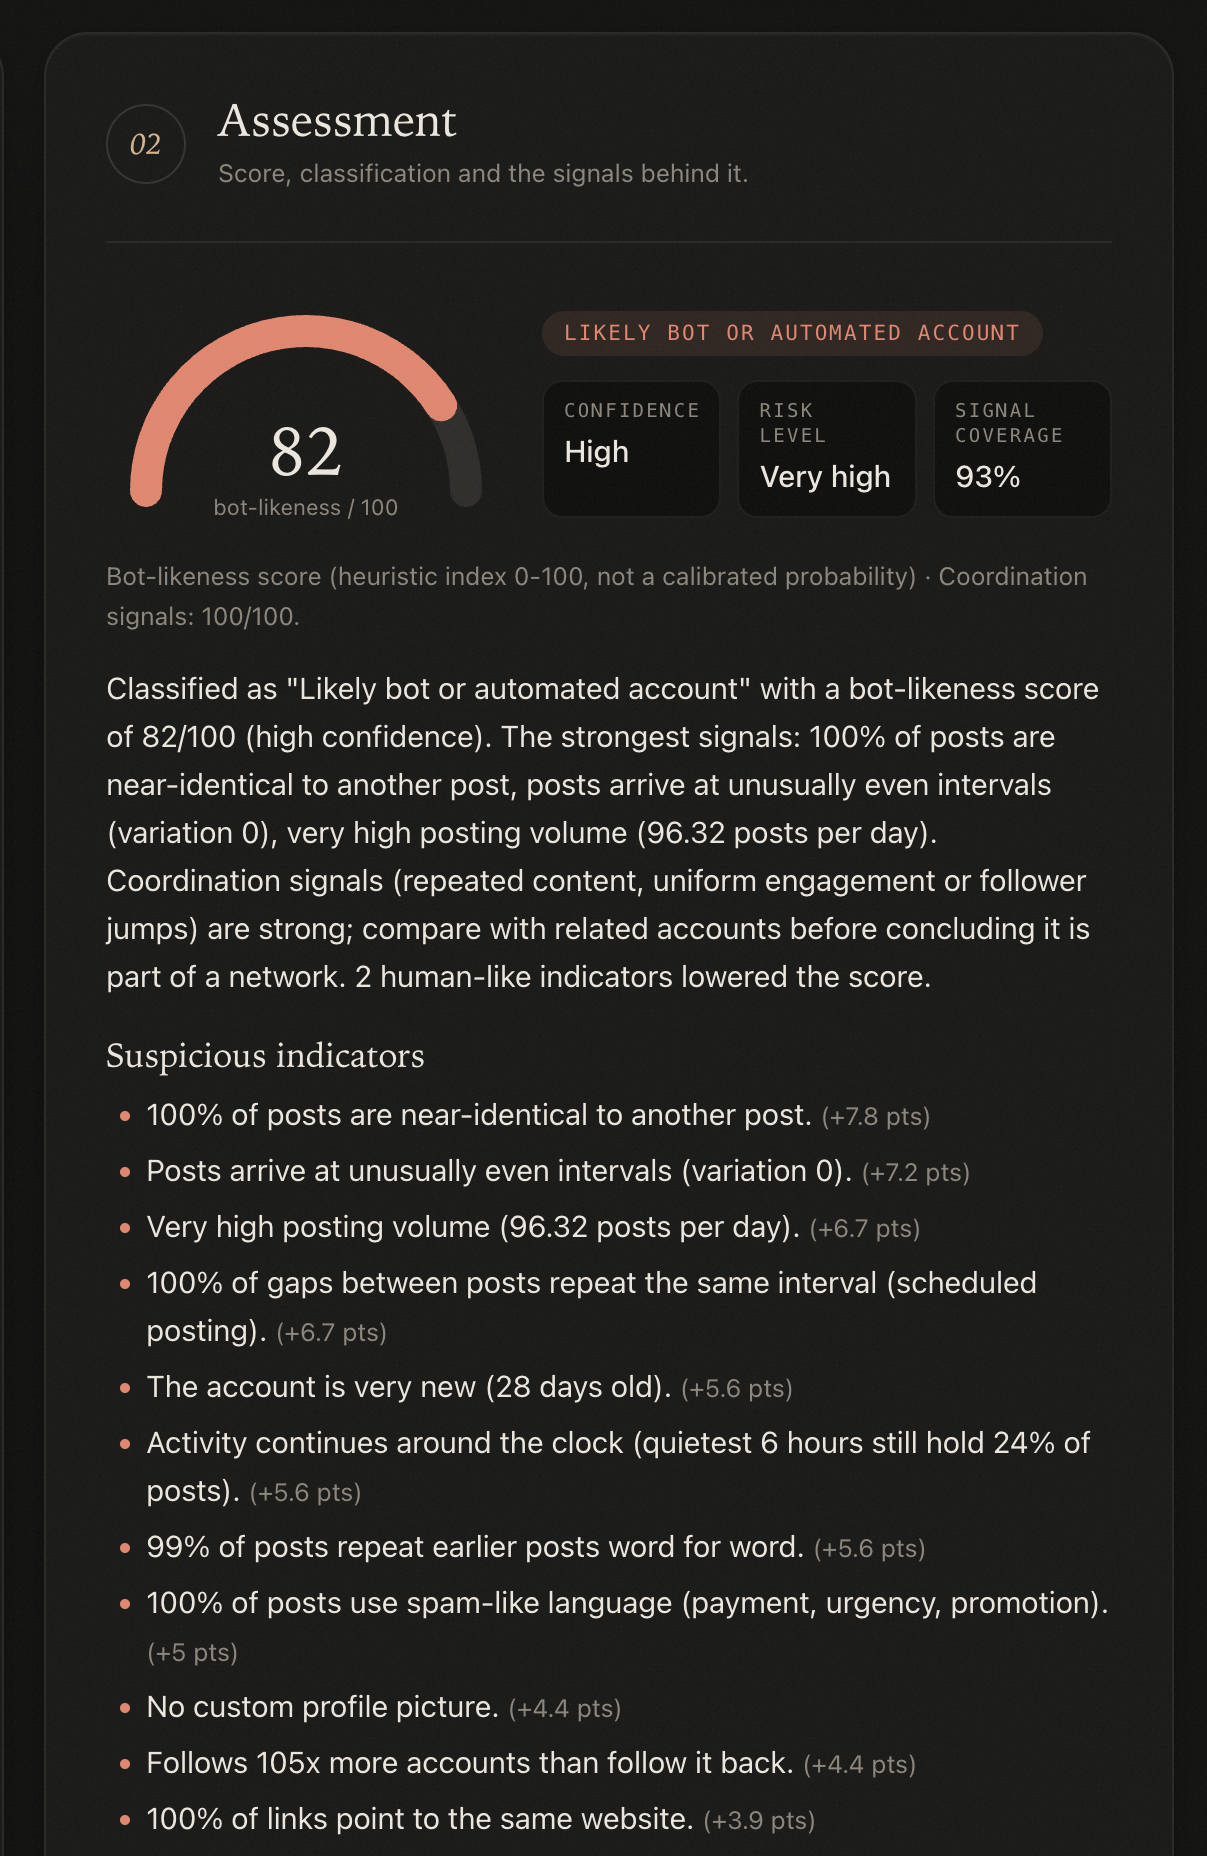
\includegraphics[width=\linewidth]{shots2/bot_report_panel.png}\\[1pt]{\small (a) Bot accounts page: assessment for an uploaded automated account (TC-28; lower part cropped)}
\end{minipage}\hfill
\begin{minipage}[t]{0.56\linewidth}\centering
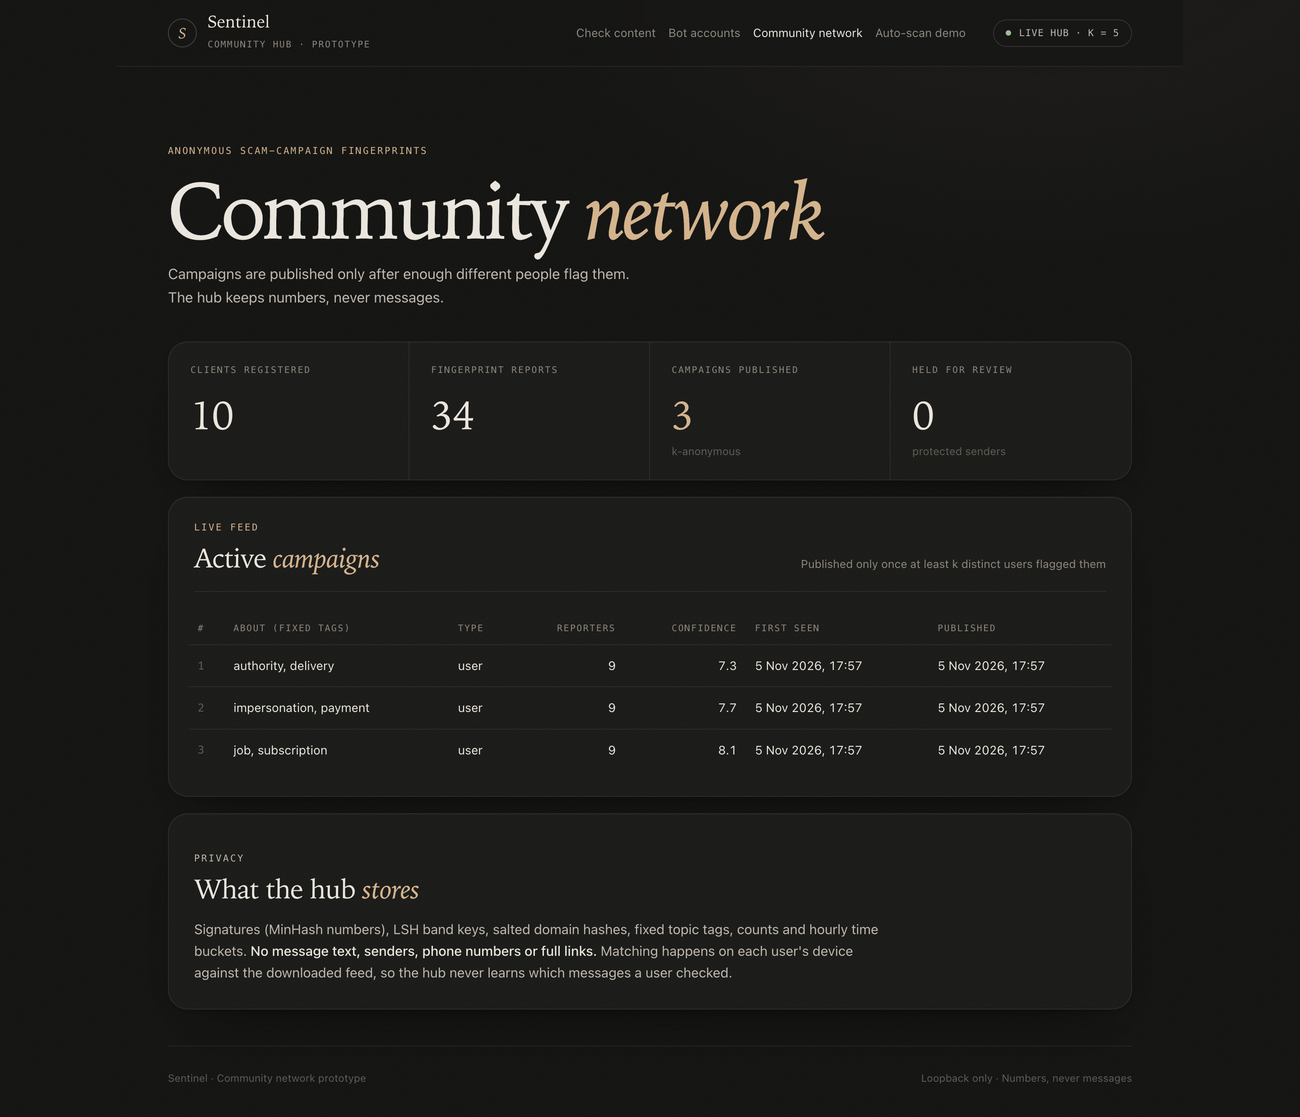
\includegraphics[width=\linewidth]{shots2/network.png}\\[1pt]{\small (b) Community network page with a live local hub}
\end{minipage}
\caption{Bot-detection and community-network pages}
\label{fig:ui-more}
\end{figure}
